\documentclass[final]{beamer}
\usepackage{color}
\usepackage{graphicx}
\DeclareGraphicsExtensions{.eps}
\usepackage{epstopdf}
\usepackage{booktabs}
\usepackage{amsmath}
\usepackage{multicol}
\usepackage{tikz}
\usepackage[absolute,overlay,showboxes]{textpos}
\usetikzlibrary{arrows}
\setbeamertemplate{caption}{\raggedright\insertcaption\par}
\usetikzlibrary{backgrounds}%arrows, shapes, trees, 
\usetikzlibrary{positioning}
\usetikzlibrary{patterns}
\title{Overcoming Throughput Degradation in Multi-Radio Cognitive Radio Networks}
\author{
    Tanvir~Ahmed~Khan
}
\institute{
    \textbf{Supervised by:}\\ Dr.~A.~B.~M.~Alim~Al~Islam\\ Assistant Professor,\\
    Dept. of Computer Science and Engineering,\\
    Bangladesh University of Engineering and Technology,\\
    Dhaka, Bangladesh.
}
%\iffalse
\titlegraphic{
\includegraphics[width=1.5cm]{figures/BuetLogo.png}
}%\fi
%\date{October 19, 2015}
\setbeamerfont{date}{size=\tiny}%series=\bfseries,,parent=structure
\date{M.Sc. Thesis Proposal}
\addtobeamertemplate{navigation symbols}{}{%
    \usebeamerfont{footline}%
    \usebeamercolor[fg]{footline}%
    \hspace{1em}%
    \insertframenumber/\inserttotalframenumber
}
\setbeamertemplate{section in toc}[sections numbered]
%\setbeamertemplate{subsection in toc}[subsections numbered]
\begin{document}

\begin{frame}
    \titlepage
\end{frame}

\iffalse
\begin{frame}{Outline of this Presentation}
    \tableofcontents[section,subsection]
\end{frame}
\fi

%\section{Preliminaries}
\section{Motivation and Background}
%\subsection{Preliminaries}

\begin{frame}
\frametitle{Preliminaries}
\framesubtitle{Cognitive Radio Networks (CRNs)}
\begin{figure}[!htbp]
\begin{center}
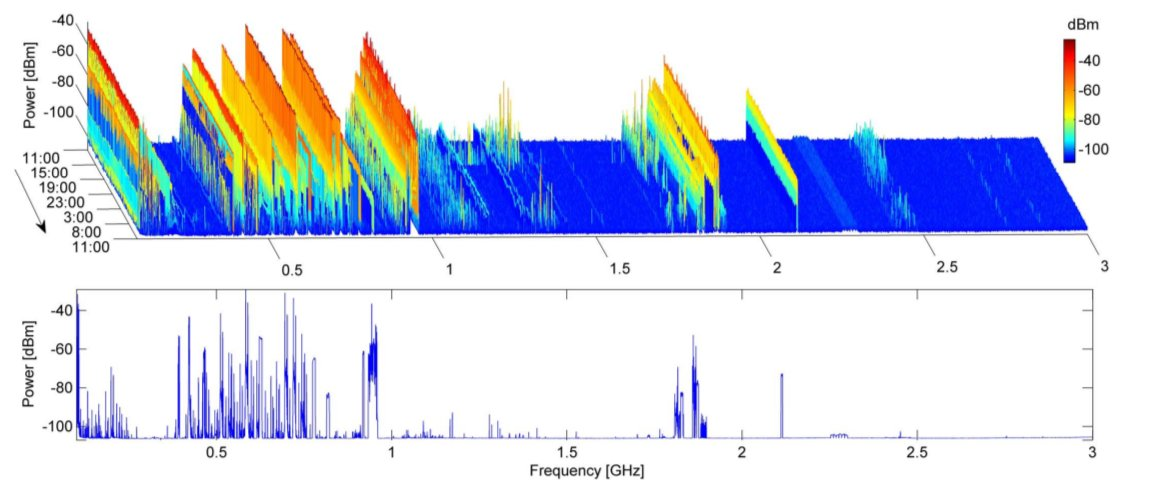
\includegraphics[scale=0.375]{figures/SpectrumUnderutilization.jpg}
%\caption{Spectrum under-utilization in traditional spectrum management~\cite{valenta2010survey}}
%\label{fig:layer}
\end{center}
\end{figure}
\begin{center}
\textcolor{red}{Licensed frequency spectrums are mostly under-utilized!~\cite{valenta2010survey}}
\end{center}
\end{frame}

\begin{frame}
\frametitle{Preliminaries}
\framesubtitle{Cognitive Radio Networks}
\noindent\begin{minipage}{\textwidth}
    \begin{minipage}[c][6cm][c]{\dimexpr0.33\textwidth-0.5\Colsep\relax}        
        \begin{subfigure}[c]{1.0\textwidth}
            
\begin{center}
    \begin{tikzpicture} [scale=0.8, transform shape]%show background rectangle,
        \tikzstyle{every node} = [draw, shape = rectangle, node distance=0mm, minimum width=5mm, minimum height=5.2mm]
        \node[draw=black, thick, label=below:Channel 2] (channel2) {
            \begin{tikzpicture}
                \node (puIdle) [fill=red!40, minimum width=30mm] {\small  Busy};%
            \end{tikzpicture}
        };
        \node[draw=black, thick, label=below:Channel 1] (channel1) [above=of channel2, yshift=7.5mm] {
            \begin{tikzpicture}
                \node (puBusy) [minimum width=30mm] {\small  Idle};
            \end{tikzpicture}
        };
        \node[draw=black, thick, label=below:Channel 3] (channel3) [below=of channel2, yshift=-7.5mm] {
            \begin{tikzpicture}
                \node (puBusy) [ minimum width=30mm] {\small  Idle};
            \end{tikzpicture}
        };
        \node[draw=black, thick, label=below:Channel 4] (channel4) [below=of channel3, yshift=-7.5mm] {
            
\begin{tikzpicture}
                \node (puBusy) [fill=red!40, minimum width=30mm] {\small  Busy};
            \end{tikzpicture}
        };

        \node[draw=white, thick] (pu1) [left=of channel1, xshift=-1mm] {
            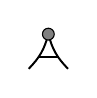
\begin{tikzpicture} [scale=0.5]
            \draw [line width=0.25mm, bend right = 15] (2, -0.44) to (2.5,0.44);
            \draw [line width=0.25mm, bend left = 15] (3, -0.44) to (2.5,0.44);
            \draw [line width=0.25mm] (2.25, -0.15) to (2.75,-0.15);
            %\draw [line width=0.25mm] (2.5, -0.44) to (2.5,0.44);
            \draw [fill=gray] (2.5,0.44) circle(1.5mm);

            \end{tikzpicture}
        };

        \node[draw=white, thick] (pu2) [left=of channel2, xshift=-1mm] {
            
\begin{tikzpicture} [scale=0.5]
            \draw [line width=0.25mm, bend right = 15, red] (2, -0.44) to (2.5,0.44);
            \draw [line width=0.25mm, bend left = 15, red] (3, -0.44) to (2.5,0.44);
            \draw [line width=0.25mm, red] (2.25, -0.15) to (2.75,-0.15);
            %\draw [line width=0.25mm] (2.5, -0.44) to (2.5,0.44);
            \draw [fill=red, red] (2.5,0.44) circle(1.5mm);

            \draw [line width=0.25mm, red] (2.5, 0.725) to (2.5,1.0);
            \draw [line width=0.25mm, red] (2.65, 0.65) to (2.825,0.85);
            \draw [line width=0.25mm, red] (2.725, 0.44) to (3,0.44);
            \draw [line width=0.25mm, red] (2.35, 0.65) to (2.175,0.85);
            \draw [line width=0.25mm, red] (2.275, 0.44) to (2,0.44);

            \end{tikzpicture}
        };

        \node[draw=white, thick] (pux1) [left=of pu2, xshift=-1mm] {
            
\begin{tikzpicture} [scale=0.5]
            \draw [line width=0.25mm, bend right = 15, red] (2, -0.44) to (2.5,0.44);
            \draw [line width=0.25mm, bend left = 15, red] (3, -0.44) to (2.5,0.44);
            \draw [line width=0.25mm, red] (2.15, -0.3) to (2.85,-0.3);
            \draw [line width=0.25mm, red] (2.25, -0.15) to (2.75,-0.15);
            \draw [line width=0.25mm, red] (2.35, 0) to (2.65,0);
            %\draw [line width=0.25mm] (2.5, -0.44) to (2.5,0.44);
            \draw [fill=red, red] (2.5,0.44) circle(1.5mm);

            \draw [line width=0.25mm, red] (2.5, 0.725) to (2.5,1.0);
            \draw [line width=0.25mm, red] (2.65, 0.65) to (2.825,0.85);
            \draw [line width=0.25mm, red] (2.725, 0.44) to (3,0.44);
            \draw [line width=0.25mm, red] (2.35, 0.65) to (2.175,0.85);
            \draw [line width=0.25mm, red] (2.275, 0.44) to (2,0.44);

            \end{tikzpicture}
        };

        \node[draw=white, thick] (pux2) [left=of pux1, xshift=-1mm] {
            
\begin{tikzpicture} [scale=0.5]
            \draw [line width=0.25mm, bend right = 15, red] (2, -0.44) to (2.5,0.44);
            \draw [line width=0.25mm, bend left = 15, red] (3, -0.44) to (2.5,0.44);
            \draw [line width=0.25mm, red] (2.15, -0.3) to (2.85,-0.3);
            \draw [line width=0.25mm, red] (2.25, -0.15) to (2.75,-0.15);
            \draw [line width=0.25mm, red] (2.35, 0) to (2.65,0);
            %\draw [line width=0.25mm] (2.5, -0.44) to (2.5,0.44);
            \draw [fill=red, red] (2.5,0.44) circle(1.5mm);

            \draw [line width=0.25mm, red] (2.5, 0.725) to (2.5,1.0);
            \draw [line width=0.25mm, red] (2.65, 0.65) to (2.825,0.85);
            \draw [line width=0.25mm, red] (2.725, 0.44) to (3,0.44);
            \draw [line width=0.25mm, red] (2.35, 0.65) to (2.175,0.85);
            \draw [line width=0.25mm, red] (2.275, 0.44) to (2,0.44);

            \end{tikzpicture}
        };

        \node[draw=white, thick] (pu3) [left=of channel3, xshift=-1mm] {
            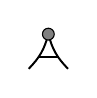
\begin{tikzpicture} [scale=0.5]
            \draw [line width=0.25mm, bend right = 15] (2, -0.44) to (2.5,0.44);
            \draw [line width=0.25mm, bend left = 15] (3, -0.44) to (2.5,0.44);
            \draw [line width=0.25mm] (2.25, -0.15) to (2.75,-0.15);
            %\draw [line width=0.25mm] (2.5, -0.44) to (2.5,0.44);
            \draw [fill=gray] (2.5,0.44) circle(1.5mm);

            \end{tikzpicture}
        };

        \node[draw=white, thick] (pu4) [left=of channel4, xshift=-1mm] {
            
\begin{tikzpicture} [scale=0.5]
            \draw [line width=0.25mm, bend right = 15, red] (2, -0.44) to (2.5,0.44);
            \draw [line width=0.25mm, bend left = 15, red] (3, -0.44) to (2.5,0.44);
            \draw [line width=0.25mm, red] (2.25, -0.15) to (2.75,-0.15);
            %\draw [line width=0.25mm] (2.5, -0.44) to (2.5,0.44);
            \draw [fill=red, red] (2.5,0.44) circle(1.5mm);

            \draw [line width=0.25mm, red] (2.5, 0.725) to (2.5,1.0);
            \draw [line width=0.25mm, red] (2.65, 0.65) to (2.825,0.85);
            \draw [line width=0.25mm, red] (2.725, 0.44) to (3,0.44);
            \draw [line width=0.25mm, red] (2.35, 0.65) to (2.175,0.85);
            \draw [line width=0.25mm, red] (2.275, 0.44) to (2,0.44);

            \end{tikzpicture}
        };
    \end{tikzpicture}
    \begin{tikzpicture}
    

        \iffalse
        \node[draw=white, thick, label=left:\tiny Primary User] (pu) [left=of pu3, xshift=-1cm] {
            \begin{tikzpicture} [scale=0.5]
            \draw [line width=0.25mm, bend right = 15] (2, -0.44) to (2.5,0.44);
            \draw [line width=0.25mm, bend left = 15] (3, -0.44) to (2.5,0.44);
            \draw [line width=0.25mm] (2.25, -0.15) to (2.75,-0.15);
            %\draw [line width=0.25mm] (2.5, -0.44) to (2.5,0.44);
            \draw [fill=gray] (2.5,0.44) circle(1.5mm);

            \end{tikzpicture}
        };

        \node[draw=white, thick] (su) [right=of su2, xshift=1cm, yshift=-1mm] {
            
\begin{tikzpicture} [scale=0.5]
            \draw [line width=0.25mm] (2, -0.44) to (2.5,0.44);
            \draw [line width=0.25mm] (3, -0.44) to (2.5,0.44);
            \draw [line width=0.25mm] (2, -0.44) to (3,-0.44);
            \draw [line width=0.25mm] (2.5, -0.44) to (2.5,0.44);
            \draw [fill=gray] (2.5,0.44) circle(1.5mm);

            \end{tikzpicture}
        };
        \fi
    \end{tikzpicture}
\begin{center}
%\only<1>{In CRNs there are some Primary users and some Secondary users, some of the Primary users remain mostly Idle, where a Secondary user can operate.}
%\only<2>{If the Idleness of a Primary user change, the Secondary user's operation can get interrupted.}
%\only<3>{The secondary user need to switch to a new Idle channel.}
%\only<4>{Now. the question is what do we focus in such CRNs?}
\end{center}
\iffalse
\only<5>{
\begin{textblock*}{0.6\textwidth}(0.28\textwidth,0.4\textheight)
\textblockcolour{green!25!white}
\centering
\vspace{5mm}
  \textcolor{red}{Motivation}\\
  significant spectrum under-utilization in traditional spectrum management~\cite{akyildiz2006next}
\vspace{5mm}
\end{textblock*}
}
\fi
\end{center}

            \label{subfig:crnPU}
        \end{subfigure}
        %
\begin{center}
    \begin{tikzpicture} [scale=0.8, transform shape]%show background rectangle,
        \tikzstyle{every node} = [draw, shape = rectangle, node distance=0mm, minimum width=5mm, minimum height=5.2mm]
        \node[draw=black, thick, label=below:Channel 2] (channel2) {
            \begin{tikzpicture}
                \node (puIdle) [fill=red!40, minimum width=30mm] {\small  Busy};%
            \end{tikzpicture}
        };
        \node[draw=black, thick, label=below:Channel 1] (channel1) [above=of channel2, yshift=7.5mm] {
            \begin{tikzpicture}
                \node (puBusy) [minimum width=30mm] {\small  Idle};
            \end{tikzpicture}
        };
        \node[draw=black, thick, label=below:Channel 3] (channel3) [below=of channel2, yshift=-7.5mm] {
            \begin{tikzpicture}
                \node (puBusy) [ minimum width=30mm] {\small  Idle};
            \end{tikzpicture}
        };
        \node[draw=black, thick, label=below:Channel 4] (channel4) [below=of channel3, yshift=-7.5mm] {
            
\begin{tikzpicture}
                \node (puBusy) [fill=red!40, minimum width=30mm] {\small  Busy};
            \end{tikzpicture}
        };

        \node[draw=white, thick] (pu1) [left=of channel1, xshift=-1mm] {
            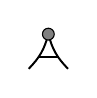
\begin{tikzpicture} [scale=0.5]
            \draw [line width=0.25mm, bend right = 15] (2, -0.44) to (2.5,0.44);
            \draw [line width=0.25mm, bend left = 15] (3, -0.44) to (2.5,0.44);
            \draw [line width=0.25mm] (2.25, -0.15) to (2.75,-0.15);
            %\draw [line width=0.25mm] (2.5, -0.44) to (2.5,0.44);
            \draw [fill=gray] (2.5,0.44) circle(1.5mm);

            \end{tikzpicture}
        };

        \node[draw=white, thick] (pu2) [left=of channel2, xshift=-1mm] {
            
\begin{tikzpicture} [scale=0.5]
            \draw [line width=0.25mm, bend right = 15, red] (2, -0.44) to (2.5,0.44);
            \draw [line width=0.25mm, bend left = 15, red] (3, -0.44) to (2.5,0.44);
            \draw [line width=0.25mm, red] (2.25, -0.15) to (2.75,-0.15);
            %\draw [line width=0.25mm] (2.5, -0.44) to (2.5,0.44);
            \draw [fill=red, red] (2.5,0.44) circle(1.5mm);

            \draw [line width=0.25mm, red] (2.5, 0.725) to (2.5,1.0);
            \draw [line width=0.25mm, red] (2.65, 0.65) to (2.825,0.85);
            \draw [line width=0.25mm, red] (2.725, 0.44) to (3,0.44);
            \draw [line width=0.25mm, red] (2.35, 0.65) to (2.175,0.85);
            \draw [line width=0.25mm, red] (2.275, 0.44) to (2,0.44);

            \end{tikzpicture}
        };

        \node[draw=white, thick] (pux1) [left=of pu2, xshift=-1mm] {
            
\begin{tikzpicture} [scale=0.5]
            \draw [line width=0.25mm, bend right = 15, red] (2, -0.44) to (2.5,0.44);
            \draw [line width=0.25mm, bend left = 15, red] (3, -0.44) to (2.5,0.44);
            \draw [line width=0.25mm, red] (2.15, -0.3) to (2.85,-0.3);
            \draw [line width=0.25mm, red] (2.25, -0.15) to (2.75,-0.15);
            \draw [line width=0.25mm, red] (2.35, 0) to (2.65,0);
            %\draw [line width=0.25mm] (2.5, -0.44) to (2.5,0.44);
            \draw [fill=red, red] (2.5,0.44) circle(1.5mm);

            \draw [line width=0.25mm, red] (2.5, 0.725) to (2.5,1.0);
            \draw [line width=0.25mm, red] (2.65, 0.65) to (2.825,0.85);
            \draw [line width=0.25mm, red] (2.725, 0.44) to (3,0.44);
            \draw [line width=0.25mm, red] (2.35, 0.65) to (2.175,0.85);
            \draw [line width=0.25mm, red] (2.275, 0.44) to (2,0.44);

            \end{tikzpicture}
        };

        \node[draw=white, thick] (pux2) [left=of pux1, xshift=-1mm] {
            
\begin{tikzpicture} [scale=0.5]
            \draw [line width=0.25mm, bend right = 15, red] (2, -0.44) to (2.5,0.44);
            \draw [line width=0.25mm, bend left = 15, red] (3, -0.44) to (2.5,0.44);
            \draw [line width=0.25mm, red] (2.15, -0.3) to (2.85,-0.3);
            \draw [line width=0.25mm, red] (2.25, -0.15) to (2.75,-0.15);
            \draw [line width=0.25mm, red] (2.35, 0) to (2.65,0);
            %\draw [line width=0.25mm] (2.5, -0.44) to (2.5,0.44);
            \draw [fill=red, red] (2.5,0.44) circle(1.5mm);

            \draw [line width=0.25mm, red] (2.5, 0.725) to (2.5,1.0);
            \draw [line width=0.25mm, red] (2.65, 0.65) to (2.825,0.85);
            \draw [line width=0.25mm, red] (2.725, 0.44) to (3,0.44);
            \draw [line width=0.25mm, red] (2.35, 0.65) to (2.175,0.85);
            \draw [line width=0.25mm, red] (2.275, 0.44) to (2,0.44);

            \end{tikzpicture}
        };

        \node[draw=white, thick] (pu3) [left=of channel3, xshift=-1mm] {
            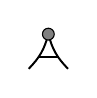
\begin{tikzpicture} [scale=0.5]
            \draw [line width=0.25mm, bend right = 15] (2, -0.44) to (2.5,0.44);
            \draw [line width=0.25mm, bend left = 15] (3, -0.44) to (2.5,0.44);
            \draw [line width=0.25mm] (2.25, -0.15) to (2.75,-0.15);
            %\draw [line width=0.25mm] (2.5, -0.44) to (2.5,0.44);
            \draw [fill=gray] (2.5,0.44) circle(1.5mm);

            \end{tikzpicture}
        };

        \node[draw=white, thick] (pu4) [left=of channel4, xshift=-1mm] {
            
\begin{tikzpicture} [scale=0.5]
            \draw [line width=0.25mm, bend right = 15, red] (2, -0.44) to (2.5,0.44);
            \draw [line width=0.25mm, bend left = 15, red] (3, -0.44) to (2.5,0.44);
            \draw [line width=0.25mm, red] (2.25, -0.15) to (2.75,-0.15);
            %\draw [line width=0.25mm] (2.5, -0.44) to (2.5,0.44);
            \draw [fill=red, red] (2.5,0.44) circle(1.5mm);

            \draw [line width=0.25mm, red] (2.5, 0.725) to (2.5,1.0);
            \draw [line width=0.25mm, red] (2.65, 0.65) to (2.825,0.85);
            \draw [line width=0.25mm, red] (2.725, 0.44) to (3,0.44);
            \draw [line width=0.25mm, red] (2.35, 0.65) to (2.175,0.85);
            \draw [line width=0.25mm, red] (2.275, 0.44) to (2,0.44);

            \end{tikzpicture}
        };
    \end{tikzpicture}
    \begin{tikzpicture}
    

        \iffalse
        \node[draw=white, thick, label=left:\tiny Primary User] (pu) [left=of pu3, xshift=-1cm] {
            \begin{tikzpicture} [scale=0.5]
            \draw [line width=0.25mm, bend right = 15] (2, -0.44) to (2.5,0.44);
            \draw [line width=0.25mm, bend left = 15] (3, -0.44) to (2.5,0.44);
            \draw [line width=0.25mm] (2.25, -0.15) to (2.75,-0.15);
            %\draw [line width=0.25mm] (2.5, -0.44) to (2.5,0.44);
            \draw [fill=gray] (2.5,0.44) circle(1.5mm);

            \end{tikzpicture}
        };

        \node[draw=white, thick] (su) [right=of su2, xshift=1cm, yshift=-1mm] {
            
\begin{tikzpicture} [scale=0.5]
            \draw [line width=0.25mm] (2, -0.44) to (2.5,0.44);
            \draw [line width=0.25mm] (3, -0.44) to (2.5,0.44);
            \draw [line width=0.25mm] (2, -0.44) to (3,-0.44);
            \draw [line width=0.25mm] (2.5, -0.44) to (2.5,0.44);
            \draw [fill=gray] (2.5,0.44) circle(1.5mm);

            \end{tikzpicture}
        };
        \fi
    \end{tikzpicture}
\begin{center}
%\only<1>{In CRNs there are some Primary users and some Secondary users, some of the Primary users remain mostly Idle, where a Secondary user can operate.}
%\only<2>{If the Idleness of a Primary user change, the Secondary user's operation can get interrupted.}
%\only<3>{The secondary user need to switch to a new Idle channel.}
%\only<4>{Now. the question is what do we focus in such CRNs?}
\end{center}
\iffalse
\only<5>{
\begin{textblock*}{0.6\textwidth}(0.28\textwidth,0.4\textheight)
\textblockcolour{green!25!white}
\centering
\vspace{5mm}
  \textcolor{red}{Motivation}\\
  significant spectrum under-utilization in traditional spectrum management~\cite{akyildiz2006next}
\vspace{5mm}
\end{textblock*}
}
\fi
\end{center}

    \end{minipage}\hfill
    \begin{minipage}[c][6cm][c]{\dimexpr0.33\textwidth-0.5\Colsep\relax}      
        \begin{subfigure}[b]{1.0\textwidth}
            
\begin{center}
    \begin{tikzpicture} [scale=0.8, transform shape]%show background rectangle,
        \tikzstyle{every node} = [draw, shape = rectangle, node distance=0mm, minimum width=5mm, minimum height=5.2mm]
        \node[draw=black, thick, label=below:Channel 2] (channel2) {
            \begin{tikzpicture}
                \node (puIdle) [fill=red!40, minimum width=30mm] {\small  Busy};%
            \end{tikzpicture}
        };
        \node[draw=black, thick, label=below:Channel 1] (channel1) [above=of channel2, yshift=7.5mm] {
            \begin{tikzpicture}
                \node (puBusy) [minimum width=30mm] {\small  Idle};
            \end{tikzpicture}
        };
        \node[draw=black, thick, label=below:Channel 3] (channel3) [below=of channel2, yshift=-7.5mm] {
            \begin{tikzpicture}
                \node (puBusy) [ minimum width=30mm] {\small  Idle};
            \end{tikzpicture}
        };
        \node[draw=black, thick, label=below:Channel 4] (channel4) [below=of channel3, yshift=-7.5mm] {
            
\begin{tikzpicture}
                \node (puBusy) [fill=red!40, minimum width=30mm] {\small  Busy};
            \end{tikzpicture}
        };

        \node[draw=white, thick] (pu1) [left=of channel1, xshift=-1mm] {
            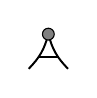
\begin{tikzpicture} [scale=0.5]
            \draw [line width=0.25mm, bend right = 15] (2, -0.44) to (2.5,0.44);
            \draw [line width=0.25mm, bend left = 15] (3, -0.44) to (2.5,0.44);
            \draw [line width=0.25mm] (2.25, -0.15) to (2.75,-0.15);
            %\draw [line width=0.25mm] (2.5, -0.44) to (2.5,0.44);
            \draw [fill=gray] (2.5,0.44) circle(1.5mm);

            \end{tikzpicture}
        };

        \node[draw=white, thick] (pu2) [left=of channel2, xshift=-1mm] {
            
\begin{tikzpicture} [scale=0.5]
            \draw [line width=0.25mm, bend right = 15, red] (2, -0.44) to (2.5,0.44);
            \draw [line width=0.25mm, bend left = 15, red] (3, -0.44) to (2.5,0.44);
            \draw [line width=0.25mm, red] (2.25, -0.15) to (2.75,-0.15);
            %\draw [line width=0.25mm] (2.5, -0.44) to (2.5,0.44);
            \draw [fill=red, red] (2.5,0.44) circle(1.5mm);

            \draw [line width=0.25mm, red] (2.5, 0.725) to (2.5,1.0);
            \draw [line width=0.25mm, red] (2.65, 0.65) to (2.825,0.85);
            \draw [line width=0.25mm, red] (2.725, 0.44) to (3,0.44);
            \draw [line width=0.25mm, red] (2.35, 0.65) to (2.175,0.85);
            \draw [line width=0.25mm, red] (2.275, 0.44) to (2,0.44);

            \end{tikzpicture}
        };

        \node[draw=white, thick] (pux1) [left=of pu2, xshift=-1mm] {
            
\begin{tikzpicture} [scale=0.5]
            \draw [line width=0.25mm, bend right = 15, red] (2, -0.44) to (2.5,0.44);
            \draw [line width=0.25mm, bend left = 15, red] (3, -0.44) to (2.5,0.44);
            \draw [line width=0.25mm, red] (2.15, -0.3) to (2.85,-0.3);
            \draw [line width=0.25mm, red] (2.25, -0.15) to (2.75,-0.15);
            \draw [line width=0.25mm, red] (2.35, 0) to (2.65,0);
            %\draw [line width=0.25mm] (2.5, -0.44) to (2.5,0.44);
            \draw [fill=red, red] (2.5,0.44) circle(1.5mm);

            \draw [line width=0.25mm, red] (2.5, 0.725) to (2.5,1.0);
            \draw [line width=0.25mm, red] (2.65, 0.65) to (2.825,0.85);
            \draw [line width=0.25mm, red] (2.725, 0.44) to (3,0.44);
            \draw [line width=0.25mm, red] (2.35, 0.65) to (2.175,0.85);
            \draw [line width=0.25mm, red] (2.275, 0.44) to (2,0.44);

            \end{tikzpicture}
        };

        \node[draw=white, thick] (pux2) [left=of pux1, xshift=-1mm] {
            
\begin{tikzpicture} [scale=0.5]
            \draw [line width=0.25mm, bend right = 15, red] (2, -0.44) to (2.5,0.44);
            \draw [line width=0.25mm, bend left = 15, red] (3, -0.44) to (2.5,0.44);
            \draw [line width=0.25mm, red] (2.15, -0.3) to (2.85,-0.3);
            \draw [line width=0.25mm, red] (2.25, -0.15) to (2.75,-0.15);
            \draw [line width=0.25mm, red] (2.35, 0) to (2.65,0);
            %\draw [line width=0.25mm] (2.5, -0.44) to (2.5,0.44);
            \draw [fill=red, red] (2.5,0.44) circle(1.5mm);

            \draw [line width=0.25mm, red] (2.5, 0.725) to (2.5,1.0);
            \draw [line width=0.25mm, red] (2.65, 0.65) to (2.825,0.85);
            \draw [line width=0.25mm, red] (2.725, 0.44) to (3,0.44);
            \draw [line width=0.25mm, red] (2.35, 0.65) to (2.175,0.85);
            \draw [line width=0.25mm, red] (2.275, 0.44) to (2,0.44);

            \end{tikzpicture}
        };
        
        \draw [line width=0.5mm, dashed, ->] (pux1) to (channel1);
        \draw [line width=0.5mm, dashed, ->] (pux2) to (channel3);

        \node[draw=white, thick] (pu3) [left=of channel3, xshift=-1mm] {
            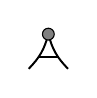
\begin{tikzpicture} [scale=0.5]
            \draw [line width=0.25mm, bend right = 15] (2, -0.44) to (2.5,0.44);
            \draw [line width=0.25mm, bend left = 15] (3, -0.44) to (2.5,0.44);
            \draw [line width=0.25mm] (2.25, -0.15) to (2.75,-0.15);
            %\draw [line width=0.25mm] (2.5, -0.44) to (2.5,0.44);
            \draw [fill=gray] (2.5,0.44) circle(1.5mm);

            \end{tikzpicture}
        };

        \node[draw=white, thick] (pu4) [left=of channel4, xshift=-1mm] {
            
\begin{tikzpicture} [scale=0.5]
            \draw [line width=0.25mm, bend right = 15, red] (2, -0.44) to (2.5,0.44);
            \draw [line width=0.25mm, bend left = 15, red] (3, -0.44) to (2.5,0.44);
            \draw [line width=0.25mm, red] (2.25, -0.15) to (2.75,-0.15);
            %\draw [line width=0.25mm] (2.5, -0.44) to (2.5,0.44);
            \draw [fill=red, red] (2.5,0.44) circle(1.5mm);

            \draw [line width=0.25mm, red] (2.5, 0.725) to (2.5,1.0);
            \draw [line width=0.25mm, red] (2.65, 0.65) to (2.825,0.85);
            \draw [line width=0.25mm, red] (2.725, 0.44) to (3,0.44);
            \draw [line width=0.25mm, red] (2.35, 0.65) to (2.175,0.85);
            \draw [line width=0.25mm, red] (2.275, 0.44) to (2,0.44);

            \end{tikzpicture}
        };
        
        
    \end{tikzpicture}
    \begin{tikzpicture}
    

        \iffalse
        \node[draw=white, thick, label=left:\tiny Primary User] (pu) [left=of pu3, xshift=-1cm] {
            \begin{tikzpicture} [scale=0.5]
            \draw [line width=0.25mm, bend right = 15] (2, -0.44) to (2.5,0.44);
            \draw [line width=0.25mm, bend left = 15] (3, -0.44) to (2.5,0.44);
            \draw [line width=0.25mm] (2.25, -0.15) to (2.75,-0.15);
            %\draw [line width=0.25mm] (2.5, -0.44) to (2.5,0.44);
            \draw [fill=gray] (2.5,0.44) circle(1.5mm);

            \end{tikzpicture}
        };

        \node[draw=white, thick] (su) [right=of su2, xshift=1cm, yshift=-1mm] {
            
\begin{tikzpicture} [scale=0.5]
            \draw [line width=0.25mm] (2, -0.44) to (2.5,0.44);
            \draw [line width=0.25mm] (3, -0.44) to (2.5,0.44);
            \draw [line width=0.25mm] (2, -0.44) to (3,-0.44);
            \draw [line width=0.25mm] (2.5, -0.44) to (2.5,0.44);
            \draw [fill=gray] (2.5,0.44) circle(1.5mm);

            \end{tikzpicture}
        };
        \fi
    \end{tikzpicture}
\begin{center}
%\only<1>{In CRNs there are some Primary users and some Secondary users, some of the Primary users remain mostly Idle, where a Secondary user can operate.}
%\only<2>{If the Idleness of a Primary user change, the Secondary user's operation can get interrupted.}
%\only<3>{The secondary user need to switch to a new Idle channel.}
%\only<4>{Now. the question is what do we focus in such CRNs?}
\end{center}
\iffalse
\only<5>{
\begin{textblock*}{0.6\textwidth}(0.28\textwidth,0.4\textheight)
\textblockcolour{green!25!white}
\centering
\vspace{5mm}
  \textcolor{red}{Motivation}\\
  significant spectrum under-utilization in traditional spectrum management~\cite{akyildiz2006next}
\vspace{5mm}
\end{textblock*}
}
\fi
\end{center}

            \label{subfig:crnPUIntermediate}
        \end{subfigure}
    \end{minipage}\hfill
    \begin{minipage}[c][6cm][c]{\dimexpr0.33\textwidth-0.5\Colsep\relax}      
        \begin{subfigure}[b]{1.0\textwidth}
            
\begin{center}
    \begin{tikzpicture} [scale=0.8, transform shape]%show background rectangle,
        \tikzstyle{every node} = [draw, shape = rectangle, node distance=0mm, minimum width=5mm, minimum height=5.2mm]
        \node[draw=black, thick, label=below:Channel 2] (channel2) {
            \begin{tikzpicture}
                \node (puIdle) [fill=red!40, minimum width=30mm] {\small  Busy};%
            \end{tikzpicture}
        };
        \node[draw=black, thick, label=below:Channel 1] (channel1) [above=of channel2, yshift=7.5mm] {
            \begin{tikzpicture}
                \node (puBusy) [minimum width=30mm] {\small  Idle};
            \end{tikzpicture}
        };
        \node[draw=black, thick, label=below:Channel 3] (channel3) [below=of channel2, yshift=-7.5mm] {
            
\begin{tikzpicture}
                \node (puBusy) [fill=green!40, minimum width=30mm] {\small  Idle};
            \end{tikzpicture}
        };
        \node[draw=black, thick, label=below:Channel 4] (channel4) [below=of channel3, yshift=-7.5mm] {
            
\begin{tikzpicture}
                \node (puBusy) [fill=red!40, minimum width=30mm] {\small  Busy};
            \end{tikzpicture}
        };
        
        \node[draw=white, thick] (sux1) [right=of channel1, xshift=1mm] {
            
\begin{tikzpicture} [scale=0.5]
            \draw [line width=0.25mm, green!50!black] (2, -0.44) to (2.5,0.44);
            \draw [line width=0.25mm, green!50!black] (3, -0.44) to (2.5,0.44);
            \draw [line width=0.25mm, green!50!black] (2, -0.44) to (3,-0.44);
            \draw [line width=0.25mm, green!50!black] (2.5, -0.44) to (2.5,0.44);
            \draw [fill=green!50!black, green!50!black] (2.5,0.44) circle(1.5mm);

            \draw [line width=0.25mm, green!50!black] (2.5, 0.725) to (2.5,1.0);
            \draw [line width=0.25mm, green!50!black] (2.65, 0.65) to (2.825,0.85);
            \draw [line width=0.25mm, green!50!black] (2.725, 0.44) to (3,0.44);
            \draw [line width=0.25mm, green!50!black] (2.35, 0.65) to (2.175,0.85);
            \draw [line width=0.25mm, green!50!black] (2.275, 0.44) to (2,0.44);

            \end{tikzpicture}
        };

        \node[draw=white, thick] (su2) [right=of channel3, xshift=1mm] {
            
\begin{tikzpicture} [scale=0.5]
            \draw [line width=0.25mm, green!50!black] (2, -0.44) to (2.5,0.44);
            \draw [line width=0.25mm, green!50!black] (3, -0.44) to (2.5,0.44);
            \draw [line width=0.25mm, green!50!black] (2, -0.44) to (3,-0.44);
            \draw [line width=0.25mm, green!50!black] (2.5, -0.44) to (2.5,0.44);
            \draw [fill=green!50!black, green!50!black] (2.5,0.44) circle(1.5mm);

            \draw [line width=0.25mm, green!50!black] (2.5, 0.725) to (2.5,1.0);
            \draw [line width=0.25mm, green!50!black] (2.65, 0.65) to (2.825,0.85);
            \draw [line width=0.25mm, green!50!black] (2.725, 0.44) to (3,0.44);
            \draw [line width=0.25mm, green!50!black] (2.35, 0.65) to (2.175,0.85);
            \draw [line width=0.25mm, green!50!black] (2.275, 0.44) to (2,0.44);

            \end{tikzpicture}
        };

        \node[draw=white, thick] (pu1) [left=of channel1, xshift=-1mm] {
            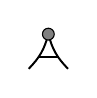
\begin{tikzpicture} [scale=0.5]
            \draw [line width=0.25mm, bend right = 15] (2, -0.44) to (2.5,0.44);
            \draw [line width=0.25mm, bend left = 15] (3, -0.44) to (2.5,0.44);
            \draw [line width=0.25mm] (2.25, -0.15) to (2.75,-0.15);
            %\draw [line width=0.25mm] (2.5, -0.44) to (2.5,0.44);
            \draw [fill=gray] (2.5,0.44) circle(1.5mm);

            \end{tikzpicture}
        };

        \node[draw=white, thick] (pu2) [left=of channel2, xshift=-1mm] {
            
\begin{tikzpicture} [scale=0.5]
            \draw [line width=0.25mm, bend right = 15, red] (2, -0.44) to (2.5,0.44);
            \draw [line width=0.25mm, bend left = 15, red] (3, -0.44) to (2.5,0.44);
            \draw [line width=0.25mm, red] (2.25, -0.15) to (2.75,-0.15);
            %\draw [line width=0.25mm] (2.5, -0.44) to (2.5,0.44);
            \draw [fill=red, red] (2.5,0.44) circle(1.5mm);

            \draw [line width=0.25mm, red] (2.5, 0.725) to (2.5,1.0);
            \draw [line width=0.25mm, red] (2.65, 0.65) to (2.825,0.85);
            \draw [line width=0.25mm, red] (2.725, 0.44) to (3,0.44);
            \draw [line width=0.25mm, red] (2.35, 0.65) to (2.175,0.85);
            \draw [line width=0.25mm, red] (2.275, 0.44) to (2,0.44);

            \end{tikzpicture}
        };

        \node[draw=white, thick] (pu3) [left=of channel3, xshift=-1mm] {
            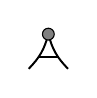
\begin{tikzpicture} [scale=0.5]
            \draw [line width=0.25mm, bend right = 15] (2, -0.44) to (2.5,0.44);
            \draw [line width=0.25mm, bend left = 15] (3, -0.44) to (2.5,0.44);
            \draw [line width=0.25mm] (2.25, -0.15) to (2.75,-0.15);
            %\draw [line width=0.25mm] (2.5, -0.44) to (2.5,0.44);
            \draw [fill=gray] (2.5,0.44) circle(1.5mm);

            \end{tikzpicture}
        };

        \node[draw=white, thick, label=below:PUs] (pu4) [left=of channel4, xshift=-1mm] {
            
\begin{tikzpicture} [scale=0.5]
            \draw [line width=0.25mm, bend right = 15, red] (2, -0.44) to (2.5,0.44);
            \draw [line width=0.25mm, bend left = 15, red] (3, -0.44) to (2.5,0.44);
            \draw [line width=0.25mm, red] (2.25, -0.15) to (2.75,-0.15);
            %\draw [line width=0.25mm] (2.5, -0.44) to (2.5,0.44);
            \draw [fill=red, red] (2.5,0.44) circle(1.5mm);

            \draw [line width=0.25mm, red] (2.5, 0.725) to (2.5,1.0);
            \draw [line width=0.25mm, red] (2.65, 0.65) to (2.825,0.85);
            \draw [line width=0.25mm, red] (2.725, 0.44) to (3,0.44);
            \draw [line width=0.25mm, red] (2.35, 0.65) to (2.175,0.85);
            \draw [line width=0.25mm, red] (2.275, 0.44) to (2,0.44);

            \end{tikzpicture}
        };

        \node[draw=white, thick, label=below:SUs] (suLabel) [right=of channel4, xshift=1mm] {
            \begin{tikzpicture} [scale=0.5]
            \draw [line width=0.25mm, white] (2, -0.44) to (2.5,0.44);
            \draw [line width=0.25mm, white] (3, -0.44) to (2.5,0.44);
            \draw [line width=0.25mm, white] (2, -0.44) to (3,-0.44);
            \draw [line width=0.25mm, white] (2.5, -0.44) to (2.5,0.44);
            \draw [fill=green!50!black, white] (2.5,0.44) circle(1.5mm);

            \draw [line width=0.25mm, white] (2.5, 0.725) to (2.5,1.0);
            \draw [line width=0.25mm, white] (2.65, 0.65) to (2.825,0.85);
            \draw [line width=0.25mm, white] (2.725, 0.44) to (3,0.44);
            \draw [line width=0.25mm, white] (2.35, 0.65) to (2.175,0.85);
            \draw [line width=0.25mm, white] (2.275, 0.44) to (2,0.44);

            \end{tikzpicture}
        };
    \end{tikzpicture}
    \begin{tikzpicture}
    

        \iffalse
        \node[draw=white, thick, label=left:\tiny Primary User] (pu) [left=of pu3, xshift=-1cm] {
            \begin{tikzpicture} [scale=0.5]
            \draw [line width=0.25mm, bend right = 15] (2, -0.44) to (2.5,0.44);
            \draw [line width=0.25mm, bend left = 15] (3, -0.44) to (2.5,0.44);
            \draw [line width=0.25mm] (2.25, -0.15) to (2.75,-0.15);
            %\draw [line width=0.25mm] (2.5, -0.44) to (2.5,0.44);
            \draw [fill=gray] (2.5,0.44) circle(1.5mm);

            \end{tikzpicture}
        };

        \node[draw=white, thick] (su) [right=of su2, xshift=1cm, yshift=-1mm] {
            
\begin{tikzpicture} [scale=0.5]
            \draw [line width=0.25mm] (2, -0.44) to (2.5,0.44);
            \draw [line width=0.25mm] (3, -0.44) to (2.5,0.44);
            \draw [line width=0.25mm] (2, -0.44) to (3,-0.44);
            \draw [line width=0.25mm] (2.5, -0.44) to (2.5,0.44);
            \draw [fill=gray] (2.5,0.44) circle(1.5mm);

            \end{tikzpicture}
        };
        \fi
    \end{tikzpicture}
\begin{center}
%\only<1>{In CRNs there are some Primary users and some Secondary users, some of the Primary users remain mostly Idle, where a Secondary user can operate.}
%\only<2>{If the Idleness of a Primary user change, the Secondary user's operation can get interrupted.}
%\only<3>{The secondary user need to switch to a new Idle channel.}
%\only<4>{Now. the question is what do we focus in such CRNs?}
\end{center}
\iffalse
\only<5>{
\begin{textblock*}{0.6\textwidth}(0.28\textwidth,0.4\textheight)
\textblockcolour{green!25!white}
\centering
\vspace{5mm}
  \textcolor{red}{Motivation}\\
  significant spectrum under-utilization in traditional spectrum management~\cite{akyildiz2006next}
\vspace{5mm}
\end{textblock*}
}
\fi
\end{center}

            \label{subfig:crnSU}
        \end{subfigure}
    \end{minipage}%
\end{minipage}

\end{frame}

%\subsection{Motivation}
\begin{frame}
\frametitle{Preliminaries}
\framesubtitle{Multi-radio Networks}
\only<1>{
        \begin{center}
        \begin{tikzpicture} [scale=1.0, transform shape]%show background rectangle,
        \tikzstyle{every node} = [draw, shape = rectangle, node distance=0mm, minimum width=4mm, minimum height=5mm]
        \node[draw=black, thick, label=below:\tiny Channel 1, minimum width=25mm] (channel1) {
        };
        \node[draw=black, thick, label=below:\tiny Channel 2, minimum width=25mm, fill=green!50] (channel2) [below=of channel1, yshift=-5mm] {
        };
        \node[draw=black, thick, label=below:\tiny Channel 3, minimum width=25mm, fill=green!50] (channel3) [below=of channel2, yshift=-5mm] {
        };
        \node[draw=black, thick, label=below:\tiny Channel 4, minimum width=25mm] (channel4) [below=of channel3, yshift=-5mm] {
        };
        \node[draw=white, thick] (su1) [left=of channel2, xshift=-1.5mm, yshift=0.5mm] {
            \begin{tikzpicture} [scale=0.5]
            \draw [line width=0.25mm, green!50!black] (2, -0.44) to (2.5,0.44);
            \draw [line width=0.25mm, green!50!black] (3, -0.44) to (2.5,0.44);
            \draw [line width=0.25mm, green!50!black] (2, -0.44) to (3,-0.44);
            \draw [line width=0.25mm, green!50!black] (2.5, -0.44) to (2.5,0.44);
            \draw [fill=green!50!black, green!50!black] (2.5,0.44) circle(1.5mm);

            \draw [line width=0.25mm, green!50!black] (2.5, 0.725) to (2.5,1.0);
            \draw [line width=0.25mm, green!50!black] (2.65, 0.65) to (2.825,0.85);
            \draw [line width=0.25mm, green!50!black] (2.725, 0.44) to (3,0.44);
            \draw [line width=0.25mm, green!50!black] (2.35, 0.65) to (2.175,0.85);
            \draw [line width=0.25mm, green!50!black] (2.275, 0.44) to (2,0.44);

            \end{tikzpicture}
        };
        \node[draw=white, thick, label=below:User] (su2) [left=of channel3, xshift=-1.5mm, yshift=0.5mm] {
            \begin{tikzpicture} [scale=0.5]
            \draw [line width=0.25mm, green!50!black] (2, -0.44) to (2.5,0.44);
            \draw [line width=0.25mm, green!50!black] (3, -0.44) to (2.5,0.44);
            \draw [line width=0.25mm, green!50!black] (2, -0.44) to (3,-0.44);
            \draw [line width=0.25mm, green!50!black] (2.5, -0.44) to (2.5,0.44);
            \draw [fill=green!50!black, green!50!black] (2.5,0.44) circle(1.5mm);

            \draw [line width=0.25mm, green!50!black] (2.5, 0.725) to (2.5,1.0);
            \draw [line width=0.25mm, green!50!black] (2.65, 0.65) to (2.825,0.85);
            \draw [line width=0.25mm, green!50!black] (2.725, 0.44) to (3,0.44);
            \draw [line width=0.25mm, green!50!black] (2.35, 0.65) to (2.175,0.85);
            \draw [line width=0.25mm, green!50!black] (2.275, 0.44) to (2,0.44);

            \end{tikzpicture}
        };
        \draw [line width=0.25mm,->] (su1) to (channel2);
        \draw [line width=0.25mm,->] (su2) to (channel3);
        
        \draw (-2.25,-2.5) -- (-2.25,-0.6) -- (-1.4,-0.6) -- (-1.4,-2.5) -- (-2.25,-2.5);
        \end{tikzpicture}
    \end{center}

}
\only<2>{
    \begin{center}
    \begin{tikzpicture} [scale=1.0, transform shape]%show background rectangle,
    \tikzstyle{every node} = [draw, shape = rectangle, node distance=0mm, minimum width=4mm, minimum height=5mm]
    \node[draw=black, thick, label=below:\tiny Channel 1, minimum width=25mm] (channel1) {
    };
    \node[draw=black, thick, label=below:\tiny Channel 2, minimum width=25mm, fill=gray!50, pattern=north west lines, pattern color=blue] (channel2) [below=of channel1, yshift=-5mm] {
    };
    \node[draw=black, thick, label=below:\tiny Channel 3, minimum width=25mm, fill=green!50] (channel3) [below=of channel2, yshift=-5mm] {
    };
    \node[draw=black, thick, label=below:\tiny Channel 4, minimum width=25mm] (channel4) [below=of channel3, yshift=-5mm] {
    };
    \node[draw=white, thick] (su1) [left=of channel2, xshift=-1.5mm, yshift=0.25mm] {
        \begin{tikzpicture} [scale=0.5]
        \draw [line width=0.25mm] (2, -0.44) to (2.5,0.44);
        \draw [line width=0.25mm] (3, -0.44) to (2.5,0.44);
        \draw [line width=0.25mm] (2, -0.44) to (3,-0.44);
        \draw [line width=0.25mm] (2.5, -0.44) to (2.5,0.44);
        \draw [fill=gray] (2.5,0.44) circle(1.5mm);

        \end{tikzpicture}
    };
    \node[draw=white, thick] (su2) [left=of channel3, xshift=-1.5mm, yshift=0.5mm] {
        \begin{tikzpicture} [scale=0.5]
        \draw [line width=0.25mm, green!50!black] (2, -0.44) to (2.5,0.44);
        \draw [line width=0.25mm, green!50!black] (3, -0.44) to (2.5,0.44);
        \draw [line width=0.25mm, green!50!black] (2, -0.44) to (3,-0.44);
        \draw [line width=0.25mm, green!50!black] (2.5, -0.44) to (2.5,0.44);
        \draw [fill=green!50!black, green!50!black] (2.5,0.44) circle(1.5mm);

        \draw [line width=0.25mm, green!50!black] (2.5, 0.725) to (2.5,1.0);
        \draw [line width=0.25mm, green!50!black] (2.65, 0.65) to (2.825,0.85);
        \draw [line width=0.25mm, green!50!black] (2.725, 0.44) to (3,0.44);
        \draw [line width=0.25mm, green!50!black] (2.35, 0.65) to (2.175,0.85);
        \draw [line width=0.25mm, green!50!black] (2.275, 0.44) to (2,0.44);

        \end{tikzpicture}
    };
    %\draw [line width=0.25mm,->] (su1) to (channel2);
    \draw [line width=0.25mm,->] (su2) to (channel3);
    
    \draw [red, line width=0.25mm] (-2.15,-1.45) -- (-1.5,-0.7);
    \draw [red, line width=0.25mm] (-2.15,-0.7) -- (-1.5,-1.45);
    
    \draw (-2.25,-2.5) -- (-2.25,-0.6) -- (-1.4,-0.6) -- (-1.4,-2.5) -- (-2.25,-2.5);
    \end{tikzpicture}
\end{center}
\begin{center}
    Enhances transmission reliability~\cite{miu2005improving}\\
    %It happens as operations over multiple radios enable overcoming a noisy channel through operating over the other available one.
\end{center}

}
\only<3>{
    \begin{center}
    \begin{tikzpicture} [scale=2.0, transform shape]%show background rectangle,
    \tikzstyle{every node} = [draw, shape = rectangle, node distance=0mm, minimum width=4mm, minimum height=5mm]
    \node[draw=black, thick, label=below:\tiny Channel 1, minimum width=25mm] (channel1) {
    };
    \node[draw=black, thick, label=below:\tiny Channel 2, minimum width=25mm, fill=green!25!black] (channel2) [below=of channel1, yshift=-5mm] {
    };
    \node[draw=black, thick, label=below:\tiny Channel 3, minimum width=25mm, fill=green!50!black] (channel3) [below=of channel2, yshift=-5mm] {
    };
    \node[draw=black, thick, label=below:\tiny Channel 4, minimum width=25mm, fill=green!75!black] (channel4) [below=of channel3, yshift=-5mm] {
    };
    \node[draw=white, thick] (su1) [left=of channel2, xshift=-1.5mm, yshift=0.5mm] {
        \begin{tikzpicture} [scale=0.5]
        \draw [line width=0.25mm, green!25!black, bend right = 15] (2, -0.44) to (2.5,0.44);
        \draw [line width=0.25mm, green!25!black, bend left = 15] (3, -0.44) to (2.5,0.44);
        \draw [line width=0.25mm, green!25!black,] (2.15, -0.3) to (2.85,-0.3);
        \draw [line width=0.25mm, green!25!black,] (2.25, -0.15) to (2.75,-0.15);
        \draw [line width=0.25mm, green!25!black,] (2.35, 0) to (2.65,0);
        %\draw [line width=0.25mm, green!50!black] (2, -0.44) to (3,-0.44);
        %\draw [line width=0.25mm, green!50!black] (2.5, -0.44) to (2.5,0.44);
        \draw [fill=green!50!black, green!25!black] (2.5,0.44) circle(1.5mm);

        \draw [line width=0.25mm, green!25!black] (2.5, 0.725) to (2.5,1.0);
        \draw [line width=0.25mm, green!25!black] (2.65, 0.65) to (2.825,0.85);
        \draw [line width=0.25mm, green!25!black] (2.725, 0.44) to (3,0.44);
        \draw [line width=0.25mm, green!25!black] (2.35, 0.65) to (2.175,0.85);
        \draw [line width=0.25mm, green!25!black] (2.275, 0.44) to (2,0.44);

        \end{tikzpicture}
    };
    \node[draw=white, thick] (su2) [left=of channel3, xshift=-1.5mm, yshift=0.5mm] {
        \begin{tikzpicture} [scale=0.5]
        \draw [line width=0.25mm, green!50!black] (2, -0.44) to (2.5,0.44);
        \draw [line width=0.25mm, green!50!black] (3, -0.44) to (2.5,0.44);
        \draw [line width=0.25mm, green!50!black] (2, -0.44) to (3,-0.44);
        \draw [line width=0.25mm, green!50!black] (2.5, -0.44) to (2.5,0.44);
        \draw [fill=green!50!black, green!50!black] (2.5,0.44) circle(1.5mm);

        \draw [line width=0.25mm, green!50!black] (2.5, 0.725) to (2.5,1.0);
        \draw [line width=0.25mm, green!50!black] (2.65, 0.65) to (2.825,0.85);
        \draw [line width=0.25mm, green!50!black] (2.725, 0.44) to (3,0.44);
        \draw [line width=0.25mm, green!50!black] (2.35, 0.65) to (2.175,0.85);
        \draw [line width=0.25mm, green!50!black] (2.275, 0.44) to (2,0.44);

        \end{tikzpicture}
    };
    \node[draw=white, thick] (su3) [left=of channel4, xshift=-1.5mm, yshift=0.5mm] {
        \begin{tikzpicture} [scale=0.5]
        \draw [fill=green!50!black, green!75!black] (2.3, -0.44) -- (2.5,0.44) -- (2.7, -0.44);
        \draw [fill=green!50!black, green!75!black] (2.5,0.44) circle(1.5mm);

        \draw [line width=0.25mm, green!75!black] (2.5, 0.725) to (2.5,1.0);
        \draw [line width=0.25mm, green!75!black] (2.65, 0.65) to (2.825,0.85);
        \draw [line width=0.25mm, green!75!black] (2.725, 0.44) to (3,0.44);
        \draw [line width=0.25mm, green!75!black] (2.35, 0.65) to (2.175,0.85);
        \draw [line width=0.25mm, green!75!black] (2.275, 0.44) to (2,0.44);

        \end{tikzpicture}
    };
    \draw [line width=0.25mm,->] (su1) to (channel2);
    \draw [line width=0.25mm,->] (su2) to (channel3);
    \draw [line width=0.25mm,->] (su3) to (channel4);
    
    \draw (-2.25,-3.5) -- (-2.25,-0.6) -- (-1.4,-0.6) -- (-1.4,-3.5) -- (-2.25,-3.5);
    \end{tikzpicture}
\end{center}

}
\end{frame}

\begin{frame}
\frametitle{Preliminaries}
\framesubtitle{Multi-radio Cognitive Radio Networks}
%\framesubtitle{in CRNs}
\noindent\begin{minipage}{\textwidth}
    \begin{minipage}[c][6cm][c]{\dimexpr0.5\textwidth-0.5\Colsep\relax}
    \begin{center}
    \begin{tikzpicture} [scale=1.0, transform shape]%show background rectangle,
        \tikzstyle{every node} = [draw, shape = rectangle, node distance=0mm, minimum width=5mm, minimum height=5.2mm]
        \node[draw=black, thick, label=below:Channel 2] (channel2) {
            \begin{tikzpicture}
                \node (puidle) [fill=red!20, minimum width=30mm] {\small Busy};%
            \end{tikzpicture}
        };
        \node[draw=black, thick, label=below:Channel 1] (channel1) [above=of channel2, yshift=7.5mm] {
            \begin{tikzpicture}
                \node (pubusy) [minimum width=30mm] {\small Idle};
            \end{tikzpicture}
        };
        \node[draw=black, thick, label=below:Channel 3] (channel3) [below=of channel2, yshift=-7.5mm] {
            \begin{tikzpicture}
                \node (pubusy) [fill=green!20, minimum width=30mm] {\small Idle};
            \end{tikzpicture}
        };
        \node[draw=black, thick, label=below:Channel 4] (channel4) [below=of channel3, yshift=-7.5mm] {
            \begin{tikzpicture}
                \node (pubusy) [fill=red!20, minimum width=30mm] {\small Busy};
            \end{tikzpicture}
        };

        \node[draw] (mrcrn) [right=of channel3, yshift=0.8cm, xshift=0.25cm] {
            \begin{tikzpicture} [scale=0.625, transform shape]
            \node[draw=white, thick] (su2) [right=of channel3, xshift=1mm] {
            \begin{tikzpicture} [scale=0.5]
            \draw [line width=0.25mm, green!50!black] (2, -0.44) to (2.5,0.44);
            \draw [line width=0.25mm, green!50!black] (3, -0.44) to (2.5,0.44);
            \draw [line width=0.25mm, green!50!black] (2, -0.44) to (3,-0.44);
            \draw [line width=0.25mm, green!50!black] (2.5, -0.44) to (2.5,0.44);
            \draw [fill=green!50!black, green!50!black] (2.5,0.44) circle(1.5mm);

            \draw [line width=0.25mm, green!50!black] (2.5, 0.725) to (2.5,1.0);
            \draw [line width=0.25mm, green!50!black] (2.65, 0.65) to (2.825,0.85);
            \draw [line width=0.25mm, green!50!black] (2.725, 0.44) to (3,0.44);
            \draw [line width=0.25mm, green!50!black] (2.35, 0.65) to (2.175,0.85);
            \draw [line width=0.25mm, green!50!black] (2.275, 0.44) to (2,0.44);

            \end{tikzpicture}
        };

        

        \node[draw=white, thick] (su3) [right=of channel2, xshift=1mm] {
            \begin{tikzpicture} [scale=0.5]
            \draw [line width=0.25mm] (2, -0.44) to (2.5,0.44);
            \draw [line width=0.25mm] (3, -0.44) to (2.5,0.44);
            \draw [line width=0.25mm] (2, -0.44) to (3,-0.44);
            \draw [line width=0.25mm] (2.5, -0.44) to (2.5,0.44);
            \draw [fill=gray] (2.5,0.44) circle(1.5mm);

            \end{tikzpicture}
        };
        
        \end{tikzpicture}
        };

        \node[draw=white, thick] (pu1) [left=of channel1, xshift=-1mm] {
            \begin{tikzpicture} [scale=0.5]
            \draw [line width=0.25mm, bend right = 15] (2, -0.44) to (2.5,0.44);
            \draw [line width=0.25mm, bend left = 15] (3, -0.44) to (2.5,0.44);
            \draw [line width=0.25mm] (2.25, -0.15) to (2.75,-0.15);
            %\draw [line width=0.25mm] (2.5, -0.44) to (2.5,0.44);
            \draw [fill=gray] (2.5,0.44) circle(1.5mm);

            \end{tikzpicture}
        };

        \node[draw=white, thick] (pu2) [left=of channel2, xshift=-1mm] {
            \begin{tikzpicture} [scale=0.5]
            \draw [line width=0.25mm, bend right = 15, red] (2, -0.44) to (2.5,0.44);
            \draw [line width=0.25mm, bend left = 15, red] (3, -0.44) to (2.5,0.44);
            \draw [line width=0.25mm, red] (2.25, -0.15) to (2.75,-0.15);
            %\draw [line width=0.25mm] (2.5, -0.44) to (2.5,0.44);
            \draw [fill=red, red] (2.5,0.44) circle(1.5mm);

            \draw [line width=0.25mm, red] (2.5, 0.725) to (2.5,1.0);
            \draw [line width=0.25mm, red] (2.65, 0.65) to (2.825,0.85);
            \draw [line width=0.25mm, red] (2.725, 0.44) to (3,0.44);
            \draw [line width=0.25mm, red] (2.35, 0.65) to (2.175,0.85);
            \draw [line width=0.25mm, red] (2.275, 0.44) to (2,0.44);

            \end{tikzpicture}
        };

        \node[draw=white, thick] (pu3) [left=of channel3, xshift=-1mm] {
            \begin{tikzpicture} [scale=0.5]
            \draw [line width=0.25mm, bend right = 15] (2, -0.44) to (2.5,0.44);
            \draw [line width=0.25mm, bend left = 15] (3, -0.44) to (2.5,0.44);
            \draw [line width=0.25mm] (2.25, -0.15) to (2.75,-0.15);
            %\draw [line width=0.25mm] (2.5, -0.44) to (2.5,0.44);
            \draw [fill=gray] (2.5,0.44) circle(1.5mm);

            \end{tikzpicture}
        };

        \node[draw=white, thick] (pu4) [left=of channel4, xshift=-1mm] {
            \begin{tikzpicture} [scale=0.5]
            \draw [line width=0.25mm, bend right = 15, red] (2, -0.44) to (2.5,0.44);
            \draw [line width=0.25mm, bend left = 15, red] (3, -0.44) to (2.5,0.44);
            \draw [line width=0.25mm, red] (2.25, -0.15) to (2.75,-0.15);
            %\draw [line width=0.25mm] (2.5, -0.44) to (2.5,0.44);
            \draw [fill=red, red] (2.5,0.44) circle(1.5mm);

            \draw [line width=0.25mm, red] (2.5, 0.725) to (2.5,1.0);
            \draw [line width=0.25mm, red] (2.65, 0.65) to (2.825,0.85);
            \draw [line width=0.25mm, red] (2.725, 0.44) to (3,0.44);
            \draw [line width=0.25mm, red] (2.35, 0.65) to (2.175,0.85);
            \draw [line width=0.25mm, red] (2.275, 0.44) to (2,0.44);

            \end{tikzpicture}
        };
    \end{tikzpicture}
    \end{center}
    \end{minipage}\hfill
    \begin{minipage}[c][6cm][c]{\dimexpr0.5\textwidth-0.5\Colsep\relax}
    \begin{center}
    \begin{tikzpicture} [scale=1.0, transform shape]%show background rectangle,
        \tikzstyle{every node} = [draw, shape = rectangle, node distance=0mm, minimum width=5mm, minimum height=5.2mm]
        \node[draw=black, thick, label=below:Channel 2] (channel2) {
            \begin{tikzpicture}
                \node (puidle) [fill=green!20, minimum width=30mm] {\small Idle};%
            \end{tikzpicture}
        };
        \node[draw=black, thick, label=below:Channel 1] (channel1) [above=of channel2, yshift=7.5mm] {
            \begin{tikzpicture}
                \node (pubusy) [minimum width=30mm] {\small Idle};
            \end{tikzpicture}
        };
        \node[draw=black, thick, label=below:Channel 3] (channel3) [below=of channel2, yshift=-7.5mm] {
            \begin{tikzpicture}
                \node (pubusy) [fill=red!20, minimum width=30mm] {\small Busy};
            \end{tikzpicture}
        };
        \node[draw=black, thick, label=below:Channel 4] (channel4) [below=of channel3, yshift=-7.5mm] {
            \begin{tikzpicture}
                \node (pubusy) [fill=red!20, minimum width=30mm] {\small Busy};
            \end{tikzpicture}
        };

        \node[draw] (mrcrn) [right=of channel3, yshift=0.8cm, xshift=0.25cm] {
            \begin{tikzpicture} [scale=0.625, transform shape]

        

        \node[draw=white, thick] (su2) [right=of channel3, xshift=1mm] {
            \begin{tikzpicture} [scale=0.5]
            \draw [line width=0.25mm] (2, -0.44) to (2.5,0.44);
            \draw [line width=0.25mm] (3, -0.44) to (2.5,0.44);
            \draw [line width=0.25mm] (2, -0.44) to (3,-0.44);
            \draw [line width=0.25mm] (2.5, -0.44) to (2.5,0.44);
            \draw [fill=gray] (2.5,0.44) circle(1.5mm);

            \end{tikzpicture}
        };

        \node[draw=white, thick] (su3) [right=of channel2, xshift=1mm] {
            \begin{tikzpicture} [scale=0.5]
            \draw [line width=0.25mm, green!50!black] (2, -0.44) to (2.5,0.44);
            \draw [line width=0.25mm, green!50!black] (3, -0.44) to (2.5,0.44);
            \draw [line width=0.25mm, green!50!black] (2, -0.44) to (3,-0.44);
            \draw [line width=0.25mm, green!50!black] (2.5, -0.44) to (2.5,0.44);
            \draw [fill=green!50!black, green!50!black] (2.5,0.44) circle(1.5mm);

            \draw [line width=0.25mm, green!50!black] (2.5, 0.725) to (2.5,1.0);
            \draw [line width=0.25mm, green!50!black] (2.65, 0.65) to (2.825,0.85);
            \draw [line width=0.25mm, green!50!black] (2.725, 0.44) to (3,0.44);
            \draw [line width=0.25mm, green!50!black] (2.35, 0.65) to (2.175,0.85);
            \draw [line width=0.25mm, green!50!black] (2.275, 0.44) to (2,0.44);

            \end{tikzpicture}
        };
        \end{tikzpicture}
        };

        \node[draw=white, thick] (pu1) [left=of channel1, xshift=-1mm] {
            \begin{tikzpicture} [scale=0.5]
            \draw [line width=0.25mm, bend right = 15] (2, -0.44) to (2.5,0.44);
            \draw [line width=0.25mm, bend left = 15] (3, -0.44) to (2.5,0.44);
            \draw [line width=0.25mm] (2.25, -0.15) to (2.75,-0.15);
            %\draw [line width=0.25mm] (2.5, -0.44) to (2.5,0.44);
            \draw [fill=gray] (2.5,0.44) circle(1.5mm);

            \end{tikzpicture}
        };

        \node[draw=white, thick] (pu2) [left=of channel2, xshift=-1mm] {
            \begin{tikzpicture} [scale=0.5]
            \draw [line width=0.25mm, bend right = 15] (2, -0.44) to (2.5,0.44);
            \draw [line width=0.25mm, bend left = 15] (3, -0.44) to (2.5,0.44);
            \draw [line width=0.25mm] (2.25, -0.15) to (2.75,-0.15);
            %\draw [line width=0.25mm] (2.5, -0.44) to (2.5,0.44);
            \draw [fill=gray] (2.5,0.44) circle(1.5mm);

            \end{tikzpicture}
        };

        \node[draw=white, thick] (pu3) [left=of channel3, xshift=-1mm] {
            \begin{tikzpicture} [scale=0.5]
            \draw [line width=0.25mm, bend right = 15, red] (2, -0.44) to (2.5,0.44);
            \draw [line width=0.25mm, bend left = 15, red] (3, -0.44) to (2.5,0.44);
            \draw [line width=0.25mm, red] (2.25, -0.15) to (2.75,-0.15);
            %\draw [line width=0.25mm] (2.5, -0.44) to (2.5,0.44);
            \draw [fill=red, red] (2.5,0.44) circle(1.5mm);

            \draw [line width=0.25mm, red] (2.5, 0.725) to (2.5,1.0);
            \draw [line width=0.25mm, red] (2.65, 0.65) to (2.825,0.85);
            \draw [line width=0.25mm, red] (2.725, 0.44) to (3,0.44);
            \draw [line width=0.25mm, red] (2.35, 0.65) to (2.175,0.85);
            \draw [line width=0.25mm, red] (2.275, 0.44) to (2,0.44);

            \end{tikzpicture}
        };

        \node[draw=white, thick] (pu4) [left=of channel4, xshift=-1mm] {
            \begin{tikzpicture} [scale=0.5]
            \draw [line width=0.25mm, bend right = 15, red] (2, -0.44) to (2.5,0.44);
            \draw [line width=0.25mm, bend left = 15, red] (3, -0.44) to (2.5,0.44);
            \draw [line width=0.25mm, red] (2.25, -0.15) to (2.75,-0.15);
            %\draw [line width=0.25mm] (2.5, -0.44) to (2.5,0.44);
            \draw [fill=red, red] (2.5,0.44) circle(1.5mm);

            \draw [line width=0.25mm, red] (2.5, 0.725) to (2.5,1.0);
            \draw [line width=0.25mm, red] (2.65, 0.65) to (2.825,0.85);
            \draw [line width=0.25mm, red] (2.725, 0.44) to (3,0.44);
            \draw [line width=0.25mm, red] (2.35, 0.65) to (2.175,0.85);
            \draw [line width=0.25mm, red] (2.275, 0.44) to (2,0.44);

            \end{tikzpicture}
        };
    \end{tikzpicture}
    \end{center}
    \end{minipage}%
\end{minipage}

\end{frame}

%\subsection{Our Contributions}
\begin{frame}
\frametitle{Preliminaries}
\framesubtitle{Throughput Degradation in Multi-radio CRNs}
%\frametitle{Results}
%\framesubtitle{Our Contributions}
\only<1>{
%However, the other metric, throughput, does not go in the same way!
\begin{figure}[!htbp]
\vspace{-0.4cm}
\begin{center}
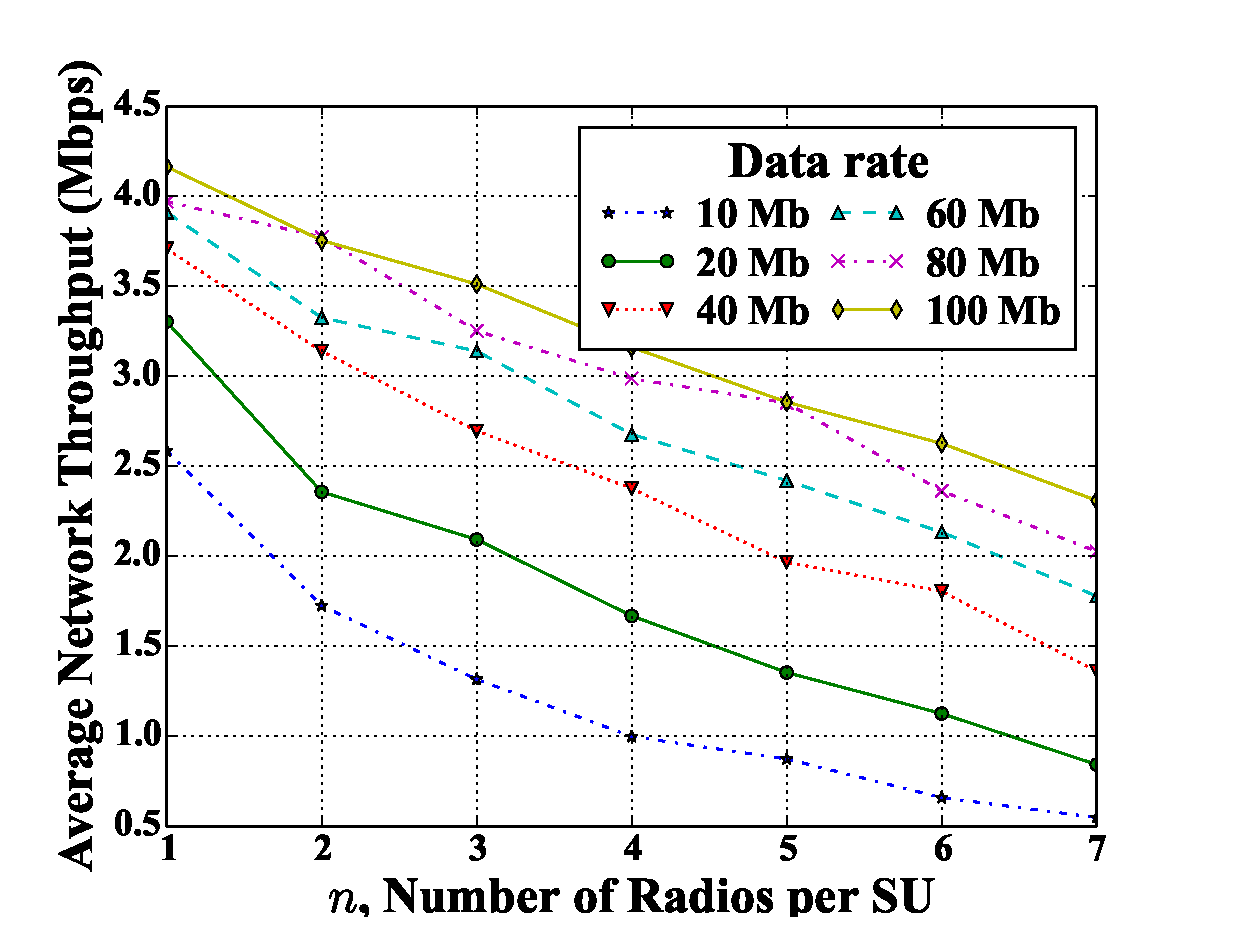
\includegraphics[scale=0.35]{figures/throughput_fragmented_datarate}
\caption{Throughput \textcolor{red}{degrades} with an increase in number of radios per SU}
\label{fig:throughput}
\end{center}
\vspace{-0.65cm}
\end{figure}
}
\only<2>{
%We start presenting outcomes of our study through experimental results first...
\begin{figure}[!htbp]
\vspace{-0.225cm}
\begin{center}
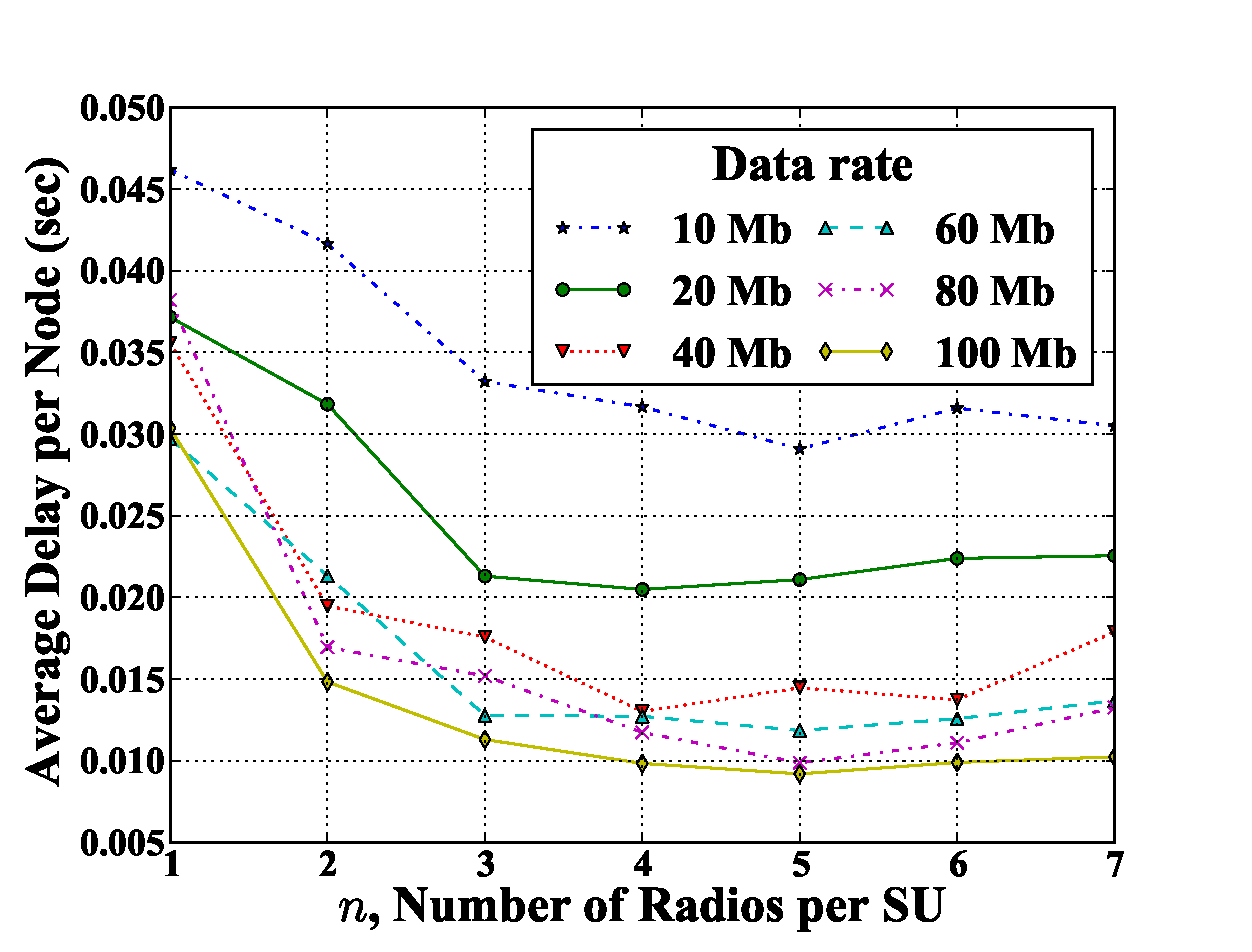
\includegraphics[scale=0.4]{figures/delay_fragmented_datarate}
\caption{Delay \textcolor{blue}{improves} up to a certain point, and then start to degrade}
%\label{fig:layer}
\end{center}
\end{figure}
}
\end{frame}

%\section{Problem Definition}
\section{Objectives \& Possible Outcome}
\begin{frame}
\frametitle{Our Research Problem}
\only<1>{
%However, the other metric, throughput, does not go in the same way!
\begin{figure}[!htbp]
%\vspace{-0.4cm}
\begin{center}
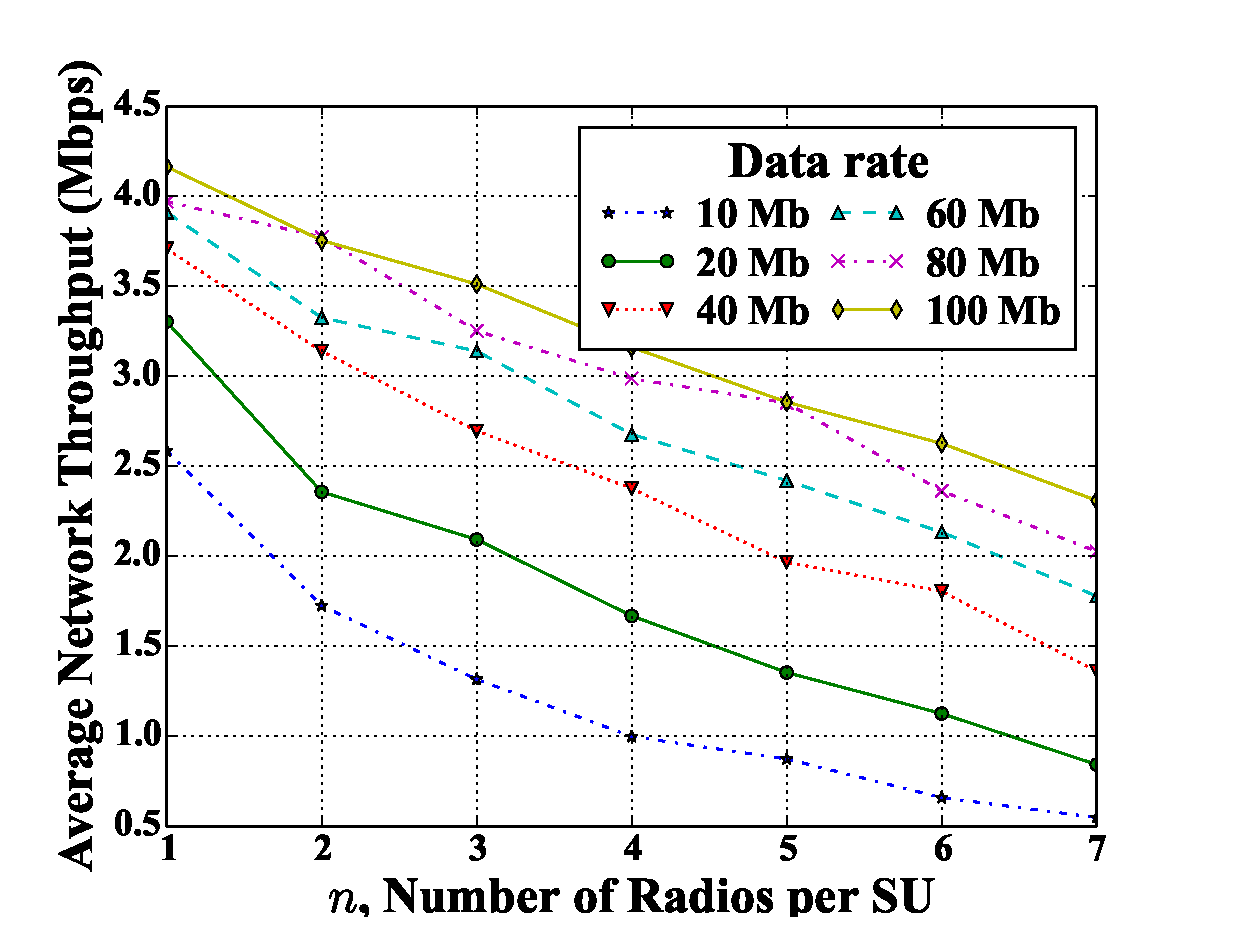
\includegraphics[scale=0.45]{figures/throughput_fragmented_datarate}
\label{fig:throughput}
\end{center}
%\vspace{-0.65cm}
\end{figure}
\begin{textblock*}{0.6\textwidth}(0.30\textwidth,0.4\textheight)
\textblockcolour{blue!15!white}
\centering
\vspace{5mm}
  %\textcolor{red}{Motivation}\\
  \textcolor{red}{How to overcome this throughput degradation in Multi-radio CRNs?}
\vspace{5mm}
\end{textblock*}
}
\only<2>{
%However, the other metric, throughput, does not go in the same way!
\begin{figure}[!htbp]
%\vspace{-0.4cm}
\begin{center}
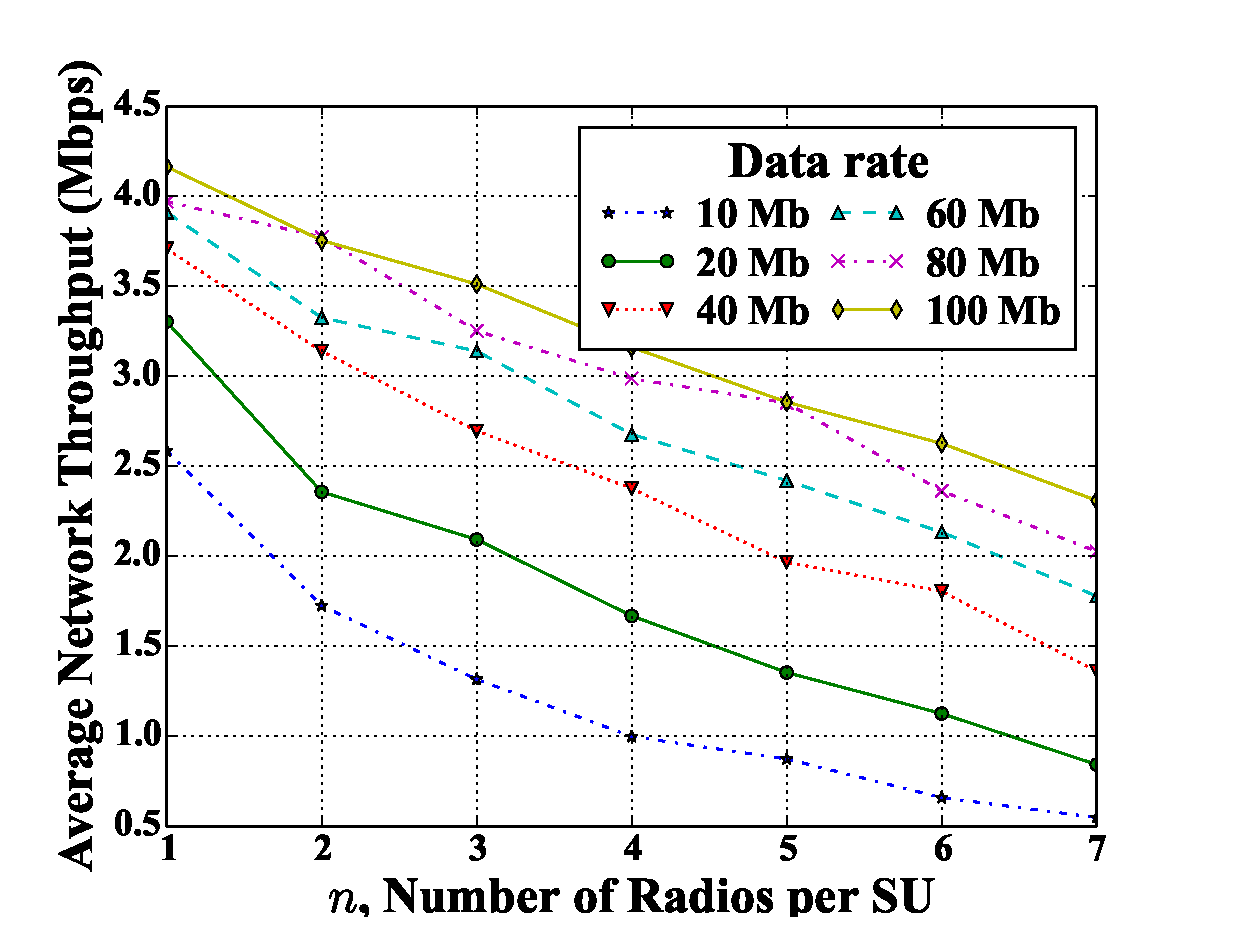
\includegraphics[scale=0.45]{figures/throughput_fragmented_datarate}
\label{fig:throughput}
\end{center}
%\vspace{-0.65cm}
\end{figure}
\begin{textblock*}{0.6\textwidth}(0.30\textwidth,0.4\textheight)
\textblockcolour{blue!15!white}
\centering
\vspace{5mm}
  %\textcolor{red}{Motivation}\\
  \textcolor{red}{More importantly, what is the reason behind this degradation?}
\vspace{5mm}
\end{textblock*}
}
\only<3>{
%However, the other metric, throughput, does not go in the same way!
\begin{figure}[!htbp]
%\vspace{-0.4cm}
\begin{center}
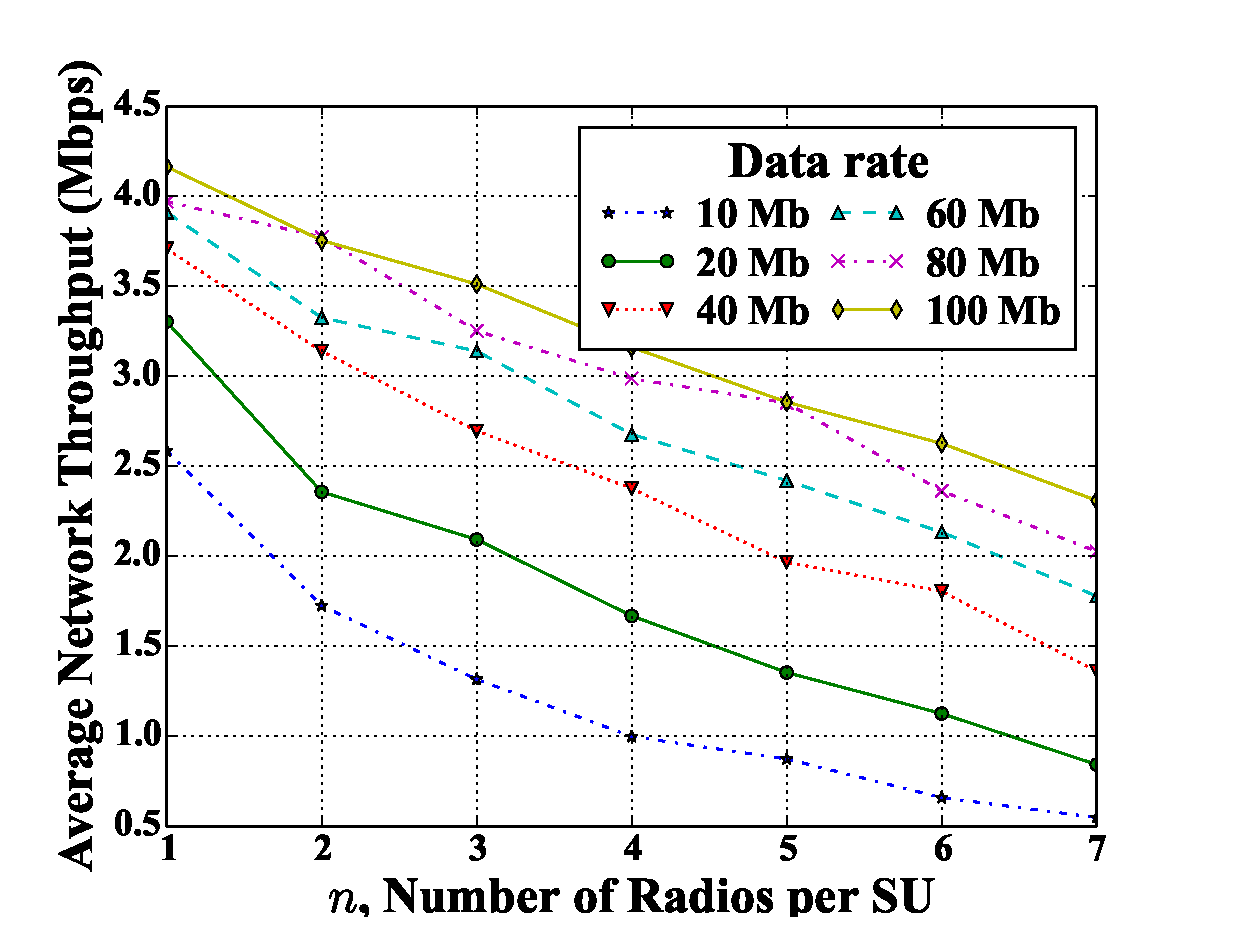
\includegraphics[scale=0.45]{figures/throughput_fragmented_datarate}
\label{fig:throughput}
\end{center}
%\vspace{-0.65cm}
\end{figure}
\begin{textblock*}{0.6\textwidth}(0.30\textwidth,0.4\textheight)
\textblockcolour{blue!15!white}
\centering
\vspace{5mm}
  %\textcolor{red}{Motivation}\\
  \textcolor{red}{Possible reason, \textbf{Intra-user radio collision}}
\vspace{5mm}
\end{textblock*}
}
\only<4>{
%However, the other metric, throughput, does not go in the same way!
\begin{figure}[!htbp]
%\vspace{-0.4cm}
\begin{center}
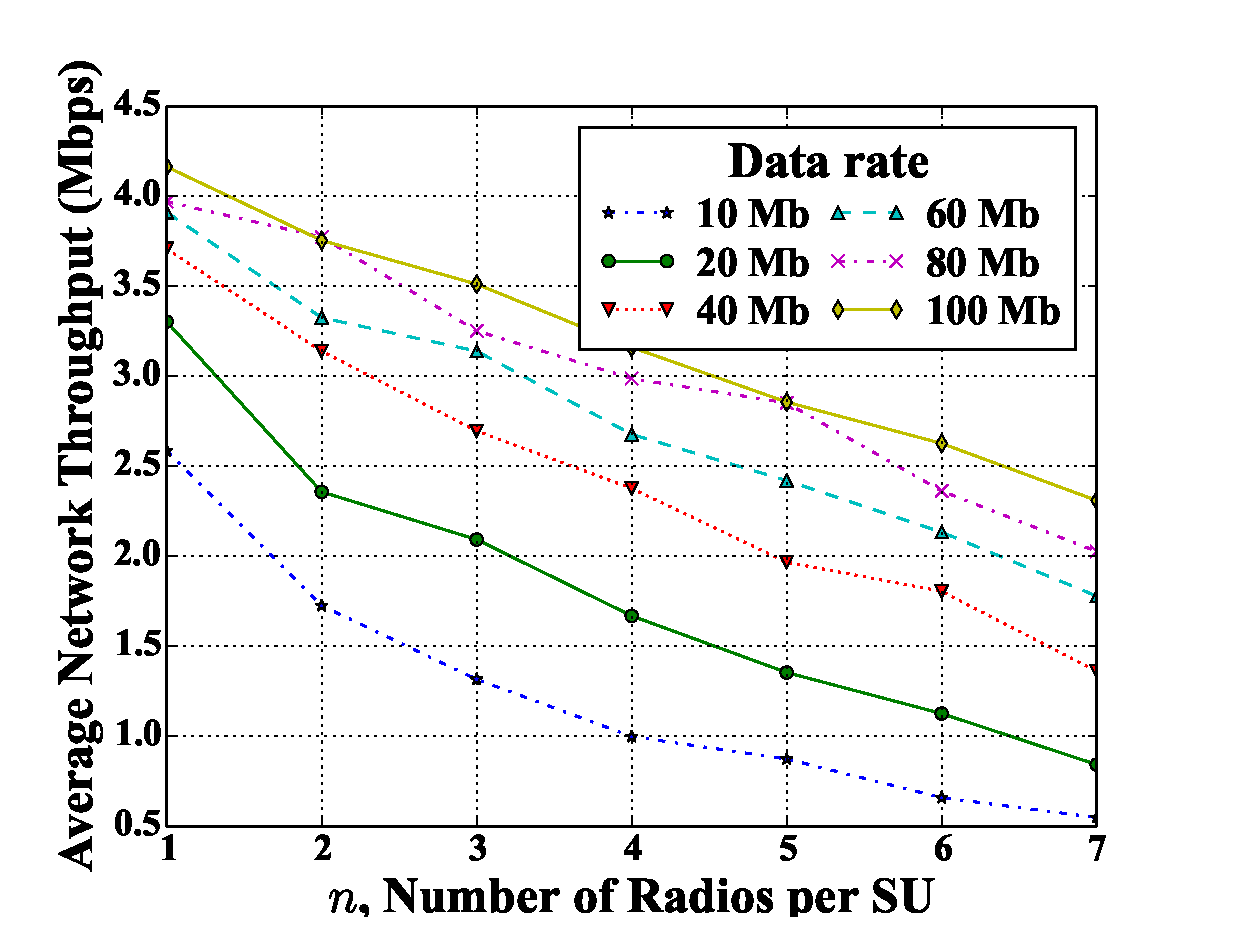
\includegraphics[scale=0.45]{figures/throughput_fragmented_datarate}
\label{fig:throughput}
\end{center}
%\vspace{-0.65cm}
\end{figure}
\begin{textblock*}{0.6\textwidth}(0.30\textwidth,0.4\textheight)
\textblockcolour{blue!15!white}
\centering
\vspace{5mm}
  %\textcolor{red}{Motivation}\\
  \textcolor{red}{How to lessen this Intra-user radio collision?}
\vspace{5mm}
\end{textblock*}
}
\only<5>{
%We start presenting outcomes of our study through experimental results first...
\begin{figure}[!htbp]
\vspace{-0.225cm}
\begin{center}
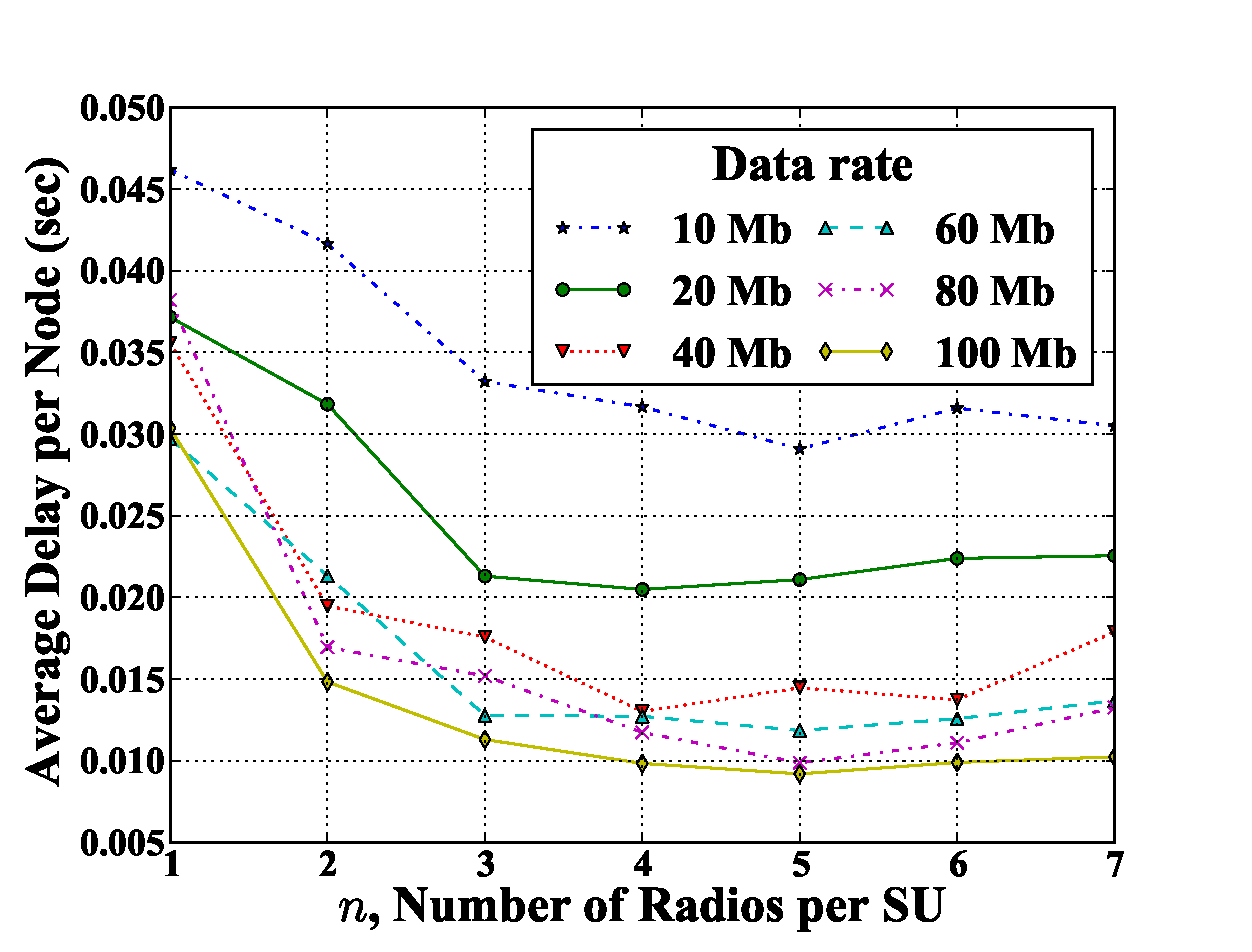
\includegraphics[scale=0.45]{figures/delay_fragmented_datarate}
%\label{fig:layer}
\end{center}
\end{figure}
\begin{textblock*}{0.72\textwidth}(0.25\textwidth,0.4\textheight)
\textblockcolour{blue!15!white}
\centering
\vspace{5mm}
  %\textcolor{red}{Motivation}\\
  \textcolor{red}{Also, we want to make sure that delay does not get worse while attempting to increase the throughput.}
\vspace{5mm}
\end{textblock*}
}
\end{frame}

\section{Outline of Methodology}
\begin{frame}
\frametitle{Our System Model}
\begin{figure}[!htbp]
\begin{center}
\begin{tikzpicture}[scale=0.8, transform shape]
    %\draw [help lines] (0, 0) grid (10, 7);
    \draw (0, 0) node {\begin{tikzpicture}[scale=1.0, transform shape]
    \node[draw=white, thick] (puRadio) {
        \begin{tikzpicture} [scale=0.5]
        \draw [line width=0.25mm, bend right = 15, red] (2, -0.44) to (2.5,0.44);
        \draw [line width=0.25mm, bend left = 15, red] (3, -0.44) to (2.5,0.44);
        \draw [line width=0.25mm, red] (2.15, -0.3) to (2.85,-0.3);
        \draw [line width=0.25mm, red] (2.25, -0.15) to (2.75,-0.15);
        \draw [line width=0.25mm, red] (2.35, 0) to (2.65,0);
        %\draw [line width=0.25mm] (2.5, -0.44) to (2.5,0.44);
        \draw [fill=red, red] (2.5,0.44) circle(1.5mm);

        \draw [line width=0.25mm, red] (2.5, 0.725) to (2.5,1.0);
        \draw [line width=0.25mm, red] (2.65, 0.65) to (2.825,0.85);
        \draw [line width=0.25mm, red] (2.725, 0.44) to (3,0.44);
        \draw [line width=0.25mm, red] (2.35, 0.65) to (2.175,0.85);
        \draw [line width=0.25mm, red] (2.275, 0.44) to (2,0.44);

        \end{tikzpicture}
    };
\end{tikzpicture}};
    \draw (0, 7) node {\begin{tikzpicture}[scale=1.0, transform shape]
    \node[draw=white, thick] (puRadio) {
        \begin{tikzpicture} [scale=0.5]
        \draw [line width=0.25mm, bend right = 15, red] (2, -0.44) to (2.5,0.44);
        \draw [line width=0.25mm, bend left = 15, red] (3, -0.44) to (2.5,0.44);
        \draw [line width=0.25mm, red] (2.15, -0.3) to (2.85,-0.3);
        \draw [line width=0.25mm, red] (2.25, -0.15) to (2.75,-0.15);
        \draw [line width=0.25mm, red] (2.35, 0) to (2.65,0);
        %\draw [line width=0.25mm] (2.5, -0.44) to (2.5,0.44);
        \draw [fill=red, red] (2.5,0.44) circle(1.5mm);

        \draw [line width=0.25mm, red] (2.5, 0.725) to (2.5,1.0);
        \draw [line width=0.25mm, red] (2.65, 0.65) to (2.825,0.85);
        \draw [line width=0.25mm, red] (2.725, 0.44) to (3,0.44);
        \draw [line width=0.25mm, red] (2.35, 0.65) to (2.175,0.85);
        \draw [line width=0.25mm, red] (2.275, 0.44) to (2,0.44);

        \end{tikzpicture}
    };
\end{tikzpicture}};
    \draw (10, 7) node {\begin{tikzpicture}[scale=1.0, transform shape]
    \node[draw=white, thick] (puRadio) {
        \begin{tikzpicture} [scale=0.5]
        \draw [line width=0.25mm, bend right = 15, red] (2, -0.44) to (2.5,0.44);
        \draw [line width=0.25mm, bend left = 15, red] (3, -0.44) to (2.5,0.44);
        \draw [line width=0.25mm, red] (2.15, -0.3) to (2.85,-0.3);
        \draw [line width=0.25mm, red] (2.25, -0.15) to (2.75,-0.15);
        \draw [line width=0.25mm, red] (2.35, 0) to (2.65,0);
        %\draw [line width=0.25mm] (2.5, -0.44) to (2.5,0.44);
        \draw [fill=red, red] (2.5,0.44) circle(1.5mm);

        \draw [line width=0.25mm, red] (2.5, 0.725) to (2.5,1.0);
        \draw [line width=0.25mm, red] (2.65, 0.65) to (2.825,0.85);
        \draw [line width=0.25mm, red] (2.725, 0.44) to (3,0.44);
        \draw [line width=0.25mm, red] (2.35, 0.65) to (2.175,0.85);
        \draw [line width=0.25mm, red] (2.275, 0.44) to (2,0.44);

        \end{tikzpicture}
    };
\end{tikzpicture}};
    \draw (10, 0) node {\begin{tikzpicture}[scale=1.0, transform shape]
    \node[draw=white, thick] (puRadio) {
        \begin{tikzpicture} [scale=0.5]
        \draw [line width=0.25mm, bend right = 15, red] (2, -0.44) to (2.5,0.44);
        \draw [line width=0.25mm, bend left = 15, red] (3, -0.44) to (2.5,0.44);
        \draw [line width=0.25mm, red] (2.15, -0.3) to (2.85,-0.3);
        \draw [line width=0.25mm, red] (2.25, -0.15) to (2.75,-0.15);
        \draw [line width=0.25mm, red] (2.35, 0) to (2.65,0);
        %\draw [line width=0.25mm] (2.5, -0.44) to (2.5,0.44);
        \draw [fill=red, red] (2.5,0.44) circle(1.5mm);

        \draw [line width=0.25mm, red] (2.5, 0.725) to (2.5,1.0);
        \draw [line width=0.25mm, red] (2.65, 0.65) to (2.825,0.85);
        \draw [line width=0.25mm, red] (2.725, 0.44) to (3,0.44);
        \draw [line width=0.25mm, red] (2.35, 0.65) to (2.175,0.85);
        \draw [line width=0.25mm, red] (2.275, 0.44) to (2,0.44);

        \end{tikzpicture}
    };
\end{tikzpicture}};
    %\draw [fill=green!50!white] (-2, -2) rectangle (2, -1);
    
    \pause
    
    \draw (5, 4.9) node {\begin{tikzpicture}[scale=1.0, transform shape]
    \tikzstyle{every node} = [draw, shape = rectangle, node distance=0mm, minimum width=4mm, minimum height=6mm, fill=green!25!white]
    \node[draw=black, thick, minimum width=25mm] (channel1) {};
\end{tikzpicture}
};
    \draw (5, 4.2) node {\begin{tikzpicture}[scale=1.0, transform shape]
    \tikzstyle{every node} = [draw, shape = rectangle, node distance=0mm, minimum width=4mm, minimum height=6mm, fill=green!25!white]
    \node[draw=black, thick, minimum width=25mm] (channel1) {};
\end{tikzpicture}
};
    \draw (5, 3.5) node {\begin{tikzpicture}[scale=1.0, transform shape]
    \tikzstyle{every node} = [draw, shape = rectangle, node distance=0mm, minimum width=4mm, minimum height=6mm, fill=green!25!white]
    \node[draw=black, thick, minimum width=25mm] (channel1) {};
\end{tikzpicture}
};
    \draw (5, 2.8) node {\begin{tikzpicture}[scale=1.0, transform shape]
    \tikzstyle{every node} = [draw, shape = rectangle, node distance=0mm, minimum width=4mm, minimum height=6mm, fill=green!25!white]
    \node[draw=black, thick, minimum width=25mm] (channel1) {};
\end{tikzpicture}
}; % [label=below:{\tiny \(n\) spectrum channels}]
    
    \pause
    
    \draw (5, 6.2) node {\begin{tikzpicture}[scale=0.375, transform shape]
    \node (controlRadio)
    {
        \begin{tikzpicture} [scale=1.0]
        \draw [fill=blue!25!white, blue!75!black] (2.3, -0.44) -- (2.5,0.44) -- (2.7, -0.44);
        \draw [fill=blue!25!white, blue!75!black] (2.5,0.44) circle(1.5mm);

        \draw [line width=0.25mm, blue!25!white] (2.5, 0.725) to (2.5,1.0);
        \draw [line width=0.25mm, blue!25!white] (2.65, 0.65) to (2.825,0.85);
        \draw [line width=0.25mm, blue!25!white] (2.725, 0.44) to (3,0.44);
        \draw [line width=0.25mm, blue!25!white] (2.35, 0.65) to (2.175,0.85);
        \draw [line width=0.25mm, blue!25!white] (2.275, 0.44) to (2,0.44);

        \end{tikzpicture}
    };
    \node (dataRadio1) [below=of controlRadio, xshift=-1.0cm, yshift=0.5cm] %, xshift=-1.5mm
    {
        \begin{tikzpicture} [scale=0.75]
        \draw [line width=0.25mm, green!50!black] (2, -0.44) to (2.5,0.44);
        \draw [line width=0.25mm, green!50!black] (3, -0.44) to (2.5,0.44);
        \draw [line width=0.25mm, green!50!black] (2, -0.44) to (3,-0.44);
        \draw [line width=0.25mm, green!50!black] (2.5, -0.44) to (2.5,0.44);
        \draw [fill=green!50!black, green!50!black] (2.5,0.44) circle(1.5mm);

        \draw [line width=0.25mm, green!50!black] (2.5, 0.725) to (2.5,1.0);
        \draw [line width=0.25mm, green!50!black] (2.65, 0.65) to (2.825,0.85);
        \draw [line width=0.25mm, green!50!black] (2.725, 0.44) to (3,0.44);
        \draw [line width=0.25mm, green!50!black] (2.35, 0.65) to (2.175,0.85);
        \draw [line width=0.25mm, green!50!black] (2.275, 0.44) to (2,0.44);

        \end{tikzpicture}
    };
    %()
    \draw[fill=green!50!black, green!50!black] (-0.25,-2.15) circle (0.025);
    \draw[fill=green!50!black, green!50!black] (0,-2.15) circle (0.025);
    \draw[fill=green!50!black, green!50!black] (0.25,-2.15) circle (0.025);
    %
    \node (dataRadio2) [right=of dataRadio1] %, xshift=-1.5mm
    {
        \begin{tikzpicture} [scale=0.75]
        \draw [line width=0.25mm, green!50!black] (2, -0.44) to (2.5,0.44);
        \draw [line width=0.25mm, green!50!black] (3, -0.44) to (2.5,0.44);
        \draw [line width=0.25mm, green!50!black] (2, -0.44) to (3,-0.44);
        \draw [line width=0.25mm, green!50!black] (2.5, -0.44) to (2.5,0.44);
        \draw [fill=green!50!black, green!50!black] (2.5,0.44) circle(1.5mm);

        \draw [line width=0.25mm, green!50!black] (2.5, 0.725) to (2.5,1.0);
        \draw [line width=0.25mm, green!50!black] (2.65, 0.65) to (2.825,0.85);
        \draw [line width=0.25mm, green!50!black] (2.725, 0.44) to (3,0.44);
        \draw [line width=0.25mm, green!50!black] (2.35, 0.65) to (2.175,0.85);
        \draw [line width=0.25mm, green!50!black] (2.275, 0.44) to (2,0.44);

        \end{tikzpicture}
    };%fill=green!50!black,
    \draw[line width=0.25mm, green!25!black] (0.25,-1) circle (3);
\end{tikzpicture}
};
    \draw (1.5, 4) node {\begin{tikzpicture}[scale=0.375, transform shape]
    \node (controlRadio)
    {
        \begin{tikzpicture} [scale=1.0]
        \draw [fill=blue!25!white, blue!75!black] (2.3, -0.44) -- (2.5,0.44) -- (2.7, -0.44);
        \draw [fill=blue!25!white, blue!75!black] (2.5,0.44) circle(1.5mm);

        \draw [line width=0.25mm, blue!25!white] (2.5, 0.725) to (2.5,1.0);
        \draw [line width=0.25mm, blue!25!white] (2.65, 0.65) to (2.825,0.85);
        \draw [line width=0.25mm, blue!25!white] (2.725, 0.44) to (3,0.44);
        \draw [line width=0.25mm, blue!25!white] (2.35, 0.65) to (2.175,0.85);
        \draw [line width=0.25mm, blue!25!white] (2.275, 0.44) to (2,0.44);

        \end{tikzpicture}
    };
    \node (dataRadio1) [below=of controlRadio, xshift=-1.0cm, yshift=0.5cm] %, xshift=-1.5mm
    {
        \begin{tikzpicture} [scale=0.75]
        \draw [line width=0.25mm, green!50!black] (2, -0.44) to (2.5,0.44);
        \draw [line width=0.25mm, green!50!black] (3, -0.44) to (2.5,0.44);
        \draw [line width=0.25mm, green!50!black] (2, -0.44) to (3,-0.44);
        \draw [line width=0.25mm, green!50!black] (2.5, -0.44) to (2.5,0.44);
        \draw [fill=green!50!black, green!50!black] (2.5,0.44) circle(1.5mm);

        \draw [line width=0.25mm, green!50!black] (2.5, 0.725) to (2.5,1.0);
        \draw [line width=0.25mm, green!50!black] (2.65, 0.65) to (2.825,0.85);
        \draw [line width=0.25mm, green!50!black] (2.725, 0.44) to (3,0.44);
        \draw [line width=0.25mm, green!50!black] (2.35, 0.65) to (2.175,0.85);
        \draw [line width=0.25mm, green!50!black] (2.275, 0.44) to (2,0.44);

        \end{tikzpicture}
    };
    %()
    \draw[fill=green!50!black, green!50!black] (-0.25,-2.15) circle (0.025);
    \draw[fill=green!50!black, green!50!black] (0,-2.15) circle (0.025);
    \draw[fill=green!50!black, green!50!black] (0.25,-2.15) circle (0.025);
    %
    \node (dataRadio2) [right=of dataRadio1] %, xshift=-1.5mm
    {
        \begin{tikzpicture} [scale=0.75]
        \draw [line width=0.25mm, green!50!black] (2, -0.44) to (2.5,0.44);
        \draw [line width=0.25mm, green!50!black] (3, -0.44) to (2.5,0.44);
        \draw [line width=0.25mm, green!50!black] (2, -0.44) to (3,-0.44);
        \draw [line width=0.25mm, green!50!black] (2.5, -0.44) to (2.5,0.44);
        \draw [fill=green!50!black, green!50!black] (2.5,0.44) circle(1.5mm);

        \draw [line width=0.25mm, green!50!black] (2.5, 0.725) to (2.5,1.0);
        \draw [line width=0.25mm, green!50!black] (2.65, 0.65) to (2.825,0.85);
        \draw [line width=0.25mm, green!50!black] (2.725, 0.44) to (3,0.44);
        \draw [line width=0.25mm, green!50!black] (2.35, 0.65) to (2.175,0.85);
        \draw [line width=0.25mm, green!50!black] (2.275, 0.44) to (2,0.44);

        \end{tikzpicture}
    };%fill=green!50!black,
    \draw[line width=0.25mm, green!25!black] (0.25,-1) circle (3);
\end{tikzpicture}
};
    \draw (2.5, 1) node {\begin{tikzpicture}[scale=0.375, transform shape]
    \node (controlRadio)
    {
        \begin{tikzpicture} [scale=1.0]
        \draw [fill=blue!25!white, blue!75!black] (2.3, -0.44) -- (2.5,0.44) -- (2.7, -0.44);
        \draw [fill=blue!25!white, blue!75!black] (2.5,0.44) circle(1.5mm);

        \draw [line width=0.25mm, blue!25!white] (2.5, 0.725) to (2.5,1.0);
        \draw [line width=0.25mm, blue!25!white] (2.65, 0.65) to (2.825,0.85);
        \draw [line width=0.25mm, blue!25!white] (2.725, 0.44) to (3,0.44);
        \draw [line width=0.25mm, blue!25!white] (2.35, 0.65) to (2.175,0.85);
        \draw [line width=0.25mm, blue!25!white] (2.275, 0.44) to (2,0.44);

        \end{tikzpicture}
    };
    \node (dataRadio1) [below=of controlRadio, xshift=-1.0cm, yshift=0.5cm] %, xshift=-1.5mm
    {
        \begin{tikzpicture} [scale=0.75]
        \draw [line width=0.25mm, green!50!black] (2, -0.44) to (2.5,0.44);
        \draw [line width=0.25mm, green!50!black] (3, -0.44) to (2.5,0.44);
        \draw [line width=0.25mm, green!50!black] (2, -0.44) to (3,-0.44);
        \draw [line width=0.25mm, green!50!black] (2.5, -0.44) to (2.5,0.44);
        \draw [fill=green!50!black, green!50!black] (2.5,0.44) circle(1.5mm);

        \draw [line width=0.25mm, green!50!black] (2.5, 0.725) to (2.5,1.0);
        \draw [line width=0.25mm, green!50!black] (2.65, 0.65) to (2.825,0.85);
        \draw [line width=0.25mm, green!50!black] (2.725, 0.44) to (3,0.44);
        \draw [line width=0.25mm, green!50!black] (2.35, 0.65) to (2.175,0.85);
        \draw [line width=0.25mm, green!50!black] (2.275, 0.44) to (2,0.44);

        \end{tikzpicture}
    };
    %()
    \draw[fill=green!50!black, green!50!black] (-0.25,-2.15) circle (0.025);
    \draw[fill=green!50!black, green!50!black] (0,-2.15) circle (0.025);
    \draw[fill=green!50!black, green!50!black] (0.25,-2.15) circle (0.025);
    %
    \node (dataRadio2) [right=of dataRadio1] %, xshift=-1.5mm
    {
        \begin{tikzpicture} [scale=0.75]
        \draw [line width=0.25mm, green!50!black] (2, -0.44) to (2.5,0.44);
        \draw [line width=0.25mm, green!50!black] (3, -0.44) to (2.5,0.44);
        \draw [line width=0.25mm, green!50!black] (2, -0.44) to (3,-0.44);
        \draw [line width=0.25mm, green!50!black] (2.5, -0.44) to (2.5,0.44);
        \draw [fill=green!50!black, green!50!black] (2.5,0.44) circle(1.5mm);

        \draw [line width=0.25mm, green!50!black] (2.5, 0.725) to (2.5,1.0);
        \draw [line width=0.25mm, green!50!black] (2.65, 0.65) to (2.825,0.85);
        \draw [line width=0.25mm, green!50!black] (2.725, 0.44) to (3,0.44);
        \draw [line width=0.25mm, green!50!black] (2.35, 0.65) to (2.175,0.85);
        \draw [line width=0.25mm, green!50!black] (2.275, 0.44) to (2,0.44);

        \end{tikzpicture}
    };%fill=green!50!black,
    \draw[line width=0.25mm, green!25!black] (0.25,-1) circle (3);
\end{tikzpicture}
};
    \draw (7.5, 1) node {\begin{tikzpicture}[scale=0.375, transform shape]
    \node (controlRadio)
    {
        \begin{tikzpicture} [scale=1.0]
        \draw [fill=blue!25!white, blue!75!black] (2.3, -0.44) -- (2.5,0.44) -- (2.7, -0.44);
        \draw [fill=blue!25!white, blue!75!black] (2.5,0.44) circle(1.5mm);

        \draw [line width=0.25mm, blue!25!white] (2.5, 0.725) to (2.5,1.0);
        \draw [line width=0.25mm, blue!25!white] (2.65, 0.65) to (2.825,0.85);
        \draw [line width=0.25mm, blue!25!white] (2.725, 0.44) to (3,0.44);
        \draw [line width=0.25mm, blue!25!white] (2.35, 0.65) to (2.175,0.85);
        \draw [line width=0.25mm, blue!25!white] (2.275, 0.44) to (2,0.44);

        \end{tikzpicture}
    };
    \node (dataRadio1) [below=of controlRadio, xshift=-1.0cm, yshift=0.5cm] %, xshift=-1.5mm
    {
        \begin{tikzpicture} [scale=0.75]
        \draw [line width=0.25mm, green!50!black] (2, -0.44) to (2.5,0.44);
        \draw [line width=0.25mm, green!50!black] (3, -0.44) to (2.5,0.44);
        \draw [line width=0.25mm, green!50!black] (2, -0.44) to (3,-0.44);
        \draw [line width=0.25mm, green!50!black] (2.5, -0.44) to (2.5,0.44);
        \draw [fill=green!50!black, green!50!black] (2.5,0.44) circle(1.5mm);

        \draw [line width=0.25mm, green!50!black] (2.5, 0.725) to (2.5,1.0);
        \draw [line width=0.25mm, green!50!black] (2.65, 0.65) to (2.825,0.85);
        \draw [line width=0.25mm, green!50!black] (2.725, 0.44) to (3,0.44);
        \draw [line width=0.25mm, green!50!black] (2.35, 0.65) to (2.175,0.85);
        \draw [line width=0.25mm, green!50!black] (2.275, 0.44) to (2,0.44);

        \end{tikzpicture}
    };
    %()
    \draw[fill=green!50!black, green!50!black] (-0.25,-2.15) circle (0.025);
    \draw[fill=green!50!black, green!50!black] (0,-2.15) circle (0.025);
    \draw[fill=green!50!black, green!50!black] (0.25,-2.15) circle (0.025);
    %
    \node (dataRadio2) [right=of dataRadio1] %, xshift=-1.5mm
    {
        \begin{tikzpicture} [scale=0.75]
        \draw [line width=0.25mm, green!50!black] (2, -0.44) to (2.5,0.44);
        \draw [line width=0.25mm, green!50!black] (3, -0.44) to (2.5,0.44);
        \draw [line width=0.25mm, green!50!black] (2, -0.44) to (3,-0.44);
        \draw [line width=0.25mm, green!50!black] (2.5, -0.44) to (2.5,0.44);
        \draw [fill=green!50!black, green!50!black] (2.5,0.44) circle(1.5mm);

        \draw [line width=0.25mm, green!50!black] (2.5, 0.725) to (2.5,1.0);
        \draw [line width=0.25mm, green!50!black] (2.65, 0.65) to (2.825,0.85);
        \draw [line width=0.25mm, green!50!black] (2.725, 0.44) to (3,0.44);
        \draw [line width=0.25mm, green!50!black] (2.35, 0.65) to (2.175,0.85);
        \draw [line width=0.25mm, green!50!black] (2.275, 0.44) to (2,0.44);

        \end{tikzpicture}
    };%fill=green!50!black,
    \draw[line width=0.25mm, green!25!black] (0.25,-1) circle (3);
\end{tikzpicture}
};
    \draw (8.5, 4) node {\begin{tikzpicture}[scale=0.375, transform shape]
    \node (controlRadio)
    {
        \begin{tikzpicture} [scale=1.0]
        \draw [fill=blue!25!white, blue!75!black] (2.3, -0.44) -- (2.5,0.44) -- (2.7, -0.44);
        \draw [fill=blue!25!white, blue!75!black] (2.5,0.44) circle(1.5mm);

        \draw [line width=0.25mm, blue!25!white] (2.5, 0.725) to (2.5,1.0);
        \draw [line width=0.25mm, blue!25!white] (2.65, 0.65) to (2.825,0.85);
        \draw [line width=0.25mm, blue!25!white] (2.725, 0.44) to (3,0.44);
        \draw [line width=0.25mm, blue!25!white] (2.35, 0.65) to (2.175,0.85);
        \draw [line width=0.25mm, blue!25!white] (2.275, 0.44) to (2,0.44);

        \end{tikzpicture}
    };
    \node (dataRadio1) [below=of controlRadio, xshift=-1.0cm, yshift=0.5cm] %, xshift=-1.5mm
    {
        \begin{tikzpicture} [scale=0.75]
        \draw [line width=0.25mm, green!50!black] (2, -0.44) to (2.5,0.44);
        \draw [line width=0.25mm, green!50!black] (3, -0.44) to (2.5,0.44);
        \draw [line width=0.25mm, green!50!black] (2, -0.44) to (3,-0.44);
        \draw [line width=0.25mm, green!50!black] (2.5, -0.44) to (2.5,0.44);
        \draw [fill=green!50!black, green!50!black] (2.5,0.44) circle(1.5mm);

        \draw [line width=0.25mm, green!50!black] (2.5, 0.725) to (2.5,1.0);
        \draw [line width=0.25mm, green!50!black] (2.65, 0.65) to (2.825,0.85);
        \draw [line width=0.25mm, green!50!black] (2.725, 0.44) to (3,0.44);
        \draw [line width=0.25mm, green!50!black] (2.35, 0.65) to (2.175,0.85);
        \draw [line width=0.25mm, green!50!black] (2.275, 0.44) to (2,0.44);

        \end{tikzpicture}
    };
    %()
    \draw[fill=green!50!black, green!50!black] (-0.25,-2.15) circle (0.025);
    \draw[fill=green!50!black, green!50!black] (0,-2.15) circle (0.025);
    \draw[fill=green!50!black, green!50!black] (0.25,-2.15) circle (0.025);
    %
    \node (dataRadio2) [right=of dataRadio1] %, xshift=-1.5mm
    {
        \begin{tikzpicture} [scale=0.75]
        \draw [line width=0.25mm, green!50!black] (2, -0.44) to (2.5,0.44);
        \draw [line width=0.25mm, green!50!black] (3, -0.44) to (2.5,0.44);
        \draw [line width=0.25mm, green!50!black] (2, -0.44) to (3,-0.44);
        \draw [line width=0.25mm, green!50!black] (2.5, -0.44) to (2.5,0.44);
        \draw [fill=green!50!black, green!50!black] (2.5,0.44) circle(1.5mm);

        \draw [line width=0.25mm, green!50!black] (2.5, 0.725) to (2.5,1.0);
        \draw [line width=0.25mm, green!50!black] (2.65, 0.65) to (2.825,0.85);
        \draw [line width=0.25mm, green!50!black] (2.725, 0.44) to (3,0.44);
        \draw [line width=0.25mm, green!50!black] (2.35, 0.65) to (2.175,0.85);
        \draw [line width=0.25mm, green!50!black] (2.275, 0.44) to (2,0.44);

        \end{tikzpicture}
    };%fill=green!50!black,
    \draw[line width=0.25mm, green!25!black] (0.25,-1) circle (3);
\end{tikzpicture}
};
    
    \pause
    
    \draw (5, 1.25) node {\begin{tikzpicture}[scale=1.0, transform shape]
    \tikzstyle{every node} = [draw, shape = rectangle, node distance=0mm, minimum width=4mm, minimum height=6mm, fill=blue!25!white]
    \node[draw=black, thick, minimum width=25mm] (channel1) {};
\end{tikzpicture}
}; % [label=below:{\tiny dedicated control channel}]
\end{tikzpicture}
\only<1>{\caption{\(n\) Primary users}}
\only<2>{\caption{\(n\) Spectrum channels}}
\only<3>{\caption{\(m\) Secondary users, each with at-least two radios}}
\only<4>{\caption{\textcolor{blue!75!white}{Dedicated control channel using a dedicated radio}}}
\end{center}
\end{figure}

\end{frame}


\begin{frame}
    \frametitle{How to Lessen Intra-user Radio Collision?}
    \framesubtitle{Radio-Channel Assignment with Collision Avoidance}
    \begin{center}
    \only<1>{
        \begin{center}
    \begin{tikzpicture} [scale=1.5, transform shape]%show background rectangle,
    \tikzstyle{every node} = [draw, shape = rectangle, node distance=0mm, minimum width=4mm, minimum height=5mm]
    \node[draw=black, thick, label=below:\tiny Channel 1, minimum width=25mm, fill=green!25] (channel1) {
    };
    \node[draw=black, thick, label=below:\tiny Channel 2, minimum width=25mm, fill=green!50] (channel2) [below=of channel1, yshift=-5mm] {
    };
    \node[draw=black, thick, label=below:\tiny Channel 3, minimum width=25mm, fill=green!75] (channel3) [below=of channel2, yshift=-5mm] {
    };
    \node[draw=black, thick, label=below:\tiny Channel 4, minimum width=25mm, fill=green!100] (channel4) [below=of channel3, yshift=-5mm] {
    };
    \node[draw=white, thick] (su1) [left=of channel2, xshift=-1.5mm, yshift=0.5mm] {
        \begin{tikzpicture} [scale=0.5]
        \draw [line width=0.25mm, green!50!black] (2, -0.44) to (2.5,0.44);
        \draw [line width=0.25mm, green!50!black] (3, -0.44) to (2.5,0.44);
        \draw [line width=0.25mm, green!50!black] (2, -0.44) to (3,-0.44);
        \draw [line width=0.25mm, green!50!black] (2.5, -0.44) to (2.5,0.44);
        \draw [fill=green!50!black, green!50!black] (2.5,0.44) circle(1.5mm);

        \draw [line width=0.25mm, green!50!black] (2.5, 0.725) to (2.5,1.0);
        \draw [line width=0.25mm, green!50!black] (2.65, 0.65) to (2.825,0.85);
        \draw [line width=0.25mm, green!50!black] (2.725, 0.44) to (3,0.44);
        \draw [line width=0.25mm, green!50!black] (2.35, 0.65) to (2.175,0.85);
        \draw [line width=0.25mm, green!50!black] (2.275, 0.44) to (2,0.44);

        \end{tikzpicture}
    };
    \node[draw=white, thick] (su2) [left=of channel3, xshift=-1.5mm, yshift=0.5mm] {
        \begin{tikzpicture} [scale=0.5]
        \draw [line width=0.25mm, green!50!black] (2, -0.44) to (2.5,0.44);
        \draw [line width=0.25mm, green!50!black] (3, -0.44) to (2.5,0.44);
        \draw [line width=0.25mm, green!50!black] (2, -0.44) to (3,-0.44);
        \draw [line width=0.25mm, green!50!black] (2.5, -0.44) to (2.5,0.44);
        \draw [fill=green!50!black, green!50!black] (2.5,0.44) circle(1.5mm);

        \draw [line width=0.25mm, green!50!black] (2.5, 0.725) to (2.5,1.0);
        \draw [line width=0.25mm, green!50!black] (2.65, 0.65) to (2.825,0.85);
        \draw [line width=0.25mm, green!50!black] (2.725, 0.44) to (3,0.44);
        \draw [line width=0.25mm, green!50!black] (2.35, 0.65) to (2.175,0.85);
        \draw [line width=0.25mm, green!50!black] (2.275, 0.44) to (2,0.44);

        \end{tikzpicture}
    };
    \draw [line width=0.25mm,->, red!75!black] (su1) to (channel1);
    \draw [line width=0.25mm,->, red!75!black] (su1) to (channel2);
    \draw [line width=0.25mm,->, red!75!black] (su1) to (channel3);
    \draw [line width=0.25mm,->, red!75!black] (su1) to (channel4);
    \draw [line width=0.25mm,->, red!75!black] (su2) to (channel1);
    \draw [line width=0.25mm,->, red!75!black] (su2) to (channel2);
    \draw [line width=0.25mm,->, red!75!black] (su2) to (channel3);
    \draw [line width=0.25mm,->, red!75!black] (su2) to (channel4);
    
    \draw (-2.25,-2.5) -- (-2.25,-0.6) -- (-1.4,-0.6) -- (-1.4,-2.5) -- (-2.25,-2.5);
    \end{tikzpicture}
\end{center}

    }
    \only<2,3,4>{
        \begin{center}
    \begin{tikzpicture} [scale=1.5, transform shape]%show background rectangle,
    \tikzstyle{every node} = [draw, shape = rectangle, node distance=0mm, minimum width=4mm, minimum height=5mm]
    \node[draw=black, thick, label=below:\tiny Channel 1, minimum width=25mm, fill=green!25] (channel1) {
    };
    \node[draw=black, thick, label=below:\tiny Channel 2, minimum width=25mm, fill=green!50] (channel2) [below=of channel1, yshift=-5mm] {
    };
    \node[draw=black, thick, label=below:\tiny Channel 3, minimum width=25mm, fill=green!75] (channel3) [below=of channel2, yshift=-5mm] {
    };
    \node[draw=black, thick, label=below:\tiny Channel 4, minimum width=25mm, fill=green!100] (channel4) [below=of channel3, yshift=-5mm] {
    };
    \node[draw=white, thick] (su1) [left=of channel2, xshift=-1.5mm, yshift=0.5mm] {
        \begin{tikzpicture} [scale=0.5]
        \draw [line width=0.25mm, green!50!black] (2, -0.44) to (2.5,0.44);
        \draw [line width=0.25mm, green!50!black] (3, -0.44) to (2.5,0.44);
        \draw [line width=0.25mm, green!50!black] (2, -0.44) to (3,-0.44);
        \draw [line width=0.25mm, green!50!black] (2.5, -0.44) to (2.5,0.44);
        \draw [fill=green!50!black, green!50!black] (2.5,0.44) circle(1.5mm);

        \draw [line width=0.25mm, green!50!black] (2.5, 0.725) to (2.5,1.0);
        \draw [line width=0.25mm, green!50!black] (2.65, 0.65) to (2.825,0.85);
        \draw [line width=0.25mm, green!50!black] (2.725, 0.44) to (3,0.44);
        \draw [line width=0.25mm, green!50!black] (2.35, 0.65) to (2.175,0.85);
        \draw [line width=0.25mm, green!50!black] (2.275, 0.44) to (2,0.44);

        \end{tikzpicture}
    };
    \node[draw=white, thick] (su2) [left=of channel3, xshift=-1.5mm, yshift=0.5mm] {
        \begin{tikzpicture} [scale=0.5]
        \draw [line width=0.25mm, green!50!black] (2, -0.44) to (2.5,0.44);
        \draw [line width=0.25mm, green!50!black] (3, -0.44) to (2.5,0.44);
        \draw [line width=0.25mm, green!50!black] (2, -0.44) to (3,-0.44);
        \draw [line width=0.25mm, green!50!black] (2.5, -0.44) to (2.5,0.44);
        \draw [fill=green!50!black, green!50!black] (2.5,0.44) circle(1.5mm);

        \draw [line width=0.25mm, green!50!black] (2.5, 0.725) to (2.5,1.0);
        \draw [line width=0.25mm, green!50!black] (2.65, 0.65) to (2.825,0.85);
        \draw [line width=0.25mm, green!50!black] (2.725, 0.44) to (3,0.44);
        \draw [line width=0.25mm, green!50!black] (2.35, 0.65) to (2.175,0.85);
        \draw [line width=0.25mm, green!50!black] (2.275, 0.44) to (2,0.44);

        \end{tikzpicture}
    };
    \draw [line width=0.25mm,->, green!75!black] (su1) to (channel1);
    \draw [line width=0.25mm,->, green!75!black] (su1) to (channel2);
    \draw [line width=0.25mm,->, green!75!black] (su2) to (channel3);
    \draw [line width=0.25mm,->, green!75!black] (su2) to (channel4);
    
    \draw (-2.25,-2.5) -- (-2.25,-0.6) -- (-1.4,-0.6) -- (-1.4,-2.5) -- (-2.25,-2.5);
    \end{tikzpicture}
\end{center}

    }
    \end{center}
    \only<3>{
    \begin{textblock*}{0.6\textwidth}(0.30\textwidth,0.4\textheight)
    \textblockcolour{blue!15!white}
    \centering
    \vspace{5mm}
      %\textcolor{red}{Motivation}\\
      should reduce contention probability
    \vspace{5mm}
    \end{textblock*}
    }
    \only<4>{
    \pause
    \begin{textblock*}{0.6\textwidth}(0.30\textwidth,0.4\textheight)
    \textblockcolour{blue!15!white}
    \centering
    \vspace{5mm}
      %\textcolor{red}{Motivation}\\
      should also reduce switching delay
    \vspace{5mm}
    \end{textblock*}
    }
\end{frame}

\begin{frame}
    \frametitle{Feedback-based Multi-radio Exploitation}
    \begin{center}
    send data through someone who is reliable\\
    \only<1>{\chapter{Proposed Methodology: Feedback-based Multi-radio Exploitation Approach}\label{chap:feedback}

Our proposed approach consists of mainly two different types of feedbacks. Firstly, we measure packet transmission ratio for each radio to evaluate radio performance. Secondly, we calculate channel utilization ratio for each channel to assess corresponding channel condition.

\section{Overview of The Proposed Approach}

We present a brief overview of our proposed feedback-based approach in \cref{fig:overview}. As SUs are equipped with multiple radios, a single radio is first selected to send an application layer packet. The radio selection process as described in \cref{sec:radioSelect} is based on packet transmission ratio. The selected radio then senses the PU activity on its current channel. If the current channel is idle, it transmits the packet following an standard CSMA-CA protocol. However, if the current channel is busy, then the radio selects another channel and starts switching to that channel. The channel selection process is based on channel utilization ratio and is described in \cref{sec:channelSelect}.

\iffalse
\begin{figure}[!htb]
\begin{center}
%\resizebox{0.625\textwidth}{!}{
\begin{center}

\end{center}
%}
\caption{High-level overview of the proposed approach}
\label{fig:overview}
\end{center}
\end{figure}
\fi

\begin{figure}[!htb]
\begin{center}
\begin{tikzpicture}[scale=1.0, transform shape]
    \node {\begin{tikzpicture}[node distance=2cm, scale=1.0, transform shape]
\tikzset{every node/.style={text width=4cm}}
\tikzstyle{startstop} = [rectangle, rounded corners, minimum width=3cm, minimum height=1cm,text centered, draw=black, fill=red!30]
\tikzstyle{io} = [trapezium, trapezium left angle=70, trapezium right angle=110, minimum width=3cm, minimum height=1cm, text centered, draw=black, fill=blue!30]
\tikzstyle{process} = [rectangle, minimum width=3cm, minimum height=1cm, text centered, draw=black, fill=orange!30]
\tikzstyle{decision} = [diamond, minimum width=1cm,  text badly centered, inner sep=0pt, draw=black, fill=green!30]
\tikzstyle{arrow} = [thick,->,>=stealth]
\node (sendPacket) [startstop] {Transport layer packet is sent to the SU agent, \texttt{sendPacket}};
\node (getSelectedRadio) [process, below of=sendPacket] {SU agent selects a radio to transmit the packet, \texttt{getSelectedRadio}};
\node (startSensing) [decision, text width=3cm, aspect=2, below of=getSelectedRadio, yshift=-1cm] {Radio senses PU's activities, \texttt{startSensing}};
\node (startSwitching) [process, text width=3.5cm, below right =0.75cm and -0.625 cm of startSensing, xshift=-0.5cm] {Radio switches its channel, \texttt{startSwitching}};
%right of=startSensing, yshift=-3cm
\node (getSelectedChannel) [process, below=0.65cm of startSwitching, xshift=-0.25cm] {SU agent selects a channel for radio, \texttt{getSelectedChannel}};
\node (transmitPacket) [process, text width=3.5cm, below left =0.75cm and -0.625 cm of startSensing] {Radio transmits the packet, \texttt{transmitPacket}};
\node (endTransmit) [decision, text width=3cm, aspect=2, below=0.5cm of transmitPacket] {Transmission end?};
\node (end) [startstop, text width=0.5cm, below of=endTransmit] {End};
\draw [arrow] (sendPacket) -- (getSelectedRadio);
\draw [arrow] (getSelectedRadio) -- (startSensing);
\draw [arrow] (transmitPacket) -- (endTransmit);
\draw [arrow] (endTransmit) -- (end);
\node at (-3, -10) {No};
\node at (-1.4, -10.75) {Yes};
\node at (-1.75, -5) {Idle};
\node at (5.2, -5) {Busy};
\draw [arrow] (-4.9,-9.575) -- (-6,-9.575) -- (-6, -3.35) -- (0, -3.35);
\draw [arrow] (-2.8,-5) -- (-3,-5) -- (-3,-6.475);
\draw [arrow] (2.8,-5) -- (3,-5) -- (3,-6.475);
\draw [arrow] (3,-8.025) --  (3,-8.675);
\draw [arrow] (4.05,-9.575) -- (5.2,-9.575) -- (5.2, -3.35) -- (0, -3.35);
\end{tikzpicture}
};
\end{tikzpicture}
\caption{High-level overview of the proposed approach}
\label{fig:overview}
\end{center}
\end{figure}

\section{Radio Selection Based on Packet Transmission Ratio}
\label{sec:radioSelect}

When SUs are equipped with multiple data transmission radios, the first issue comes into play is to select the radio for transmitting data packets. For this selection, our proposed approach maintains two counters for each radio namely \texttt{pktQueued} denoting the number of packets queued for the radio and \texttt{pktSent} denoting the number of packets already transmitted by the radio. Whenever the Application layer of an SU sends a packet for transmission to the lower layers, the secondary user agent calculates the ratio between 	\texttt{pktSent} and \texttt{pktQueued} for each radio. We define the ratio as Packet Transmission Ratio, \texttt{sentQueuedRatio}. Subsequently, we normalize values of the ratio to rank the radios in a uniform manner. A larger value of such packet transmission ratio implies that the corresponding radio has been successful to transmit more packets than others. Using these packet transmission ratios as the weights, our proposed approach conducts a weighted lottery to select radios for transmission of packets.

At the beginning of the packet transmission process, an SU's radio senses its current channel. If the cognitive radio finds that the current channel is busy, then the radio starts a channel switching process. At the beginning of the channel switching process, the SU agent lists all the channels currently not used by any radio of the corresponding SU. If no such channel can be found, the radio is reported as Off and the queued packets are discarded as dropped. Otherwise, a channel is selected from the list of available channels, \texttt{availableChannels} based on current channel utilization ratio. We present the selection process along with the definition of the channel utilization ratio next.

\section{Channel Selection Based on Channel Utilization Ratio}
\label{sec:channelSelect}

In our proposed approach, each SU keeps two counters for each channel. First, \texttt{pktTransmitted} counts the number of packets transmitted in the channel by the corresponding SU radios. Besides, \texttt{pktReceived} counts the number of packets successfully received by the corresponding receiver. The counter, \texttt{pktReceived} is incremented after reception of each acknowledgment packet. When a switching radio requires selecting a channel among \texttt{availableChannels}, the SU agent calculates the ratio between \texttt{pktReceived} and \texttt{pktTransmitted} for each channel on the list, \texttt{availableChannels}. We define the ratio as Channel Utilization Ratio, \texttt{RxTxRatio}. We normalize this ratio to rank the channels in a uniform manner. Using these channel utilization ratios as the weights, the SU agent conducts a weighted lottery to select the channel to switch over.

The last two important aspects of our feedback-based multi-radio exploitation approach are the reactivation of Off radios and probabilistic channel switching. Radios marked Off at the beginning of a channel switching process, are reactivated probabilistically by the radio selection process. While calculating packet transmission ratio from \texttt{pktSent} and \texttt{pktQueued}, in the case of Off radios, the ratio is multiplied by \texttt{wakeUpProbability} to make it less likely to be selected as the next radio for sending a packet. Though, if selected, the Off radio is reported as On and it starts its cognitive cycle through the channel sensing process. The probabilistic channel switching implies that radios do not always switch after finding their current channel busy. The channel switching process occurs at a probability of \texttt{switchingProbability}.

\begin{algorithm}
\caption{$\mathit{sendPacket}$: SU agent sending a packet, $p$}
\label{alg:sendPacket}
\begin{algorithmic}[1]
\Function{$\mathit{sendPacket}$}{}
\State $\mathit{radioIndex}\gets \mathit{getSelectedRadio}()$
\State $pktQueued[radioIndex]\gets $\Statex$ 1+\mathit{pktQueued}[\mathit{radioIndex}]$
\State $\mathit{radioStatus}[\mathit{radioIndex}]\gets \mathit{On}$
\State $\mathit{startSensing}(\mathit{radioIndex})$
\EndFunction
\end{algorithmic}
\end{algorithm}

\begin{algorithm}
\caption{$\mathit{startSensing}$: SU's radio sensing its channel}
\label{alg:startSensing}
\begin{algorithmic}[1]
\Function{$\mathit{startSensing}$}{$\mathit{radioIndex}$}
\If{$\mathit{currentChannel}[\mathit{radioIndex}]$ is $\mathit{Busy}$}
\State $\mathit{startSwitching}(\mathit{radioIndex})$
\Else
\State $\mathit{transmitPacket}(\mathit{radioIndex})$
\EndIf
\EndFunction
\end{algorithmic}
\end{algorithm}

\begin{algorithm}
\caption{$\mathit{startSwitching}$: SU's radio changing its channel}\label{alg:startSwitching}
\begin{algorithmic}[1]
\Function{$\mathit{startSwitching}$}{$\mathit{radioIndex}$}
\State Stop the switching process and \textbf{return} with the probability $(1-\mathit{switchingProbability})$
\State $\mathit{availableChannels} \gets $ all the channels currently not used by any radio of the SU
\If{$\mathit{availableChannels}=\varnothing$}
\State $\mathit{radioStatus}[\mathit{radioIndex}]\gets \mathit{Off}$
\State $\mathit{dropPacket}()$
\Else
\State $\mathit{channelIndex}\gets$\Statex$ \mathit{getSelectedChannel}(\mathit{availableChannels})$
\State $\mathit{currentChannel}[\mathit{radioIndex}] \gets \mathit{channelIndex}$
\State $\mathit{channels}[\mathit{channelIndex}] \gets \mathit{Used}$
\State $\mathit{startSensing}(\mathit{radioIndex})$
\EndIf
\EndFunction
\end{algorithmic}
\end{algorithm}

\begin{algorithm}
\caption{$\mathit{transmitPacket}$: SU's radio transmitting a packet, $p$}
\label{alg:transmitPacket}
\begin{algorithmic}[1]
\Function{$\mathit{transmitPacket}$}{$\mathit{radioIndex}$}
\State $\mathit{pktSent}[\mathit{radioIndex}]\gets \mathit{pktSent}[\mathit{radioIndex}]+1$
\State $\mathit{pktTransmitted}[\mathit{currentChannel}[\mathit{radioIndex}]]\gets$\par\hskip\algorithmicindent$\mathit{pktTransmitted}[\mathit{currentChannel}[\mathit{radioIndex}]]$\par\hskip\algorithmicindent$+1$
\State encapsulate $\mathit{radioIndex}$ within the packet, $p$ and transmit it following CSMA-CA
\EndFunction
\end{algorithmic}
\end{algorithm}
\begin{algorithm}
\caption{$\mathit{receiveAckPacket}$: SU's radio receiving an Ack packet, $p$}
\label{alg:receivePacket}
\begin{algorithmic}[1]
\Function{$\mathit{receivePacket}$}{$p$}
\State $\mathit{radioIndex} \gets $ the radio index extracted from the packet
\If{$\mathit{radioIndex}=$ current radio's index}
\State $\mathit{pktReceivedRadio}[\mathit{radioIndex}]\gets$\Statex$ \mathit{pktReceivedRadio}[\mathit{radioIndex}]+1$
\State $\mathit{pktReceived}[\mathit{currentChannel}[\mathit{radioIndex}]]\gets$\Statex$ \mathit{pktReceived}[\mathit{currentChannel}[\mathit{radioIndex}]]+1$
\EndIf
\EndFunction
\end{algorithmic}
\end{algorithm}

\begin{algorithm}
\caption{$\mathit{getSelectedRadio}$: Selects an SU radio to send a packet}
\label{alg:getSelectedRadio}
\begin{algorithmic}[1]
\Function{$\mathit{getSelectedRadio}$}{}
%\State $\mathit{radios} \gets$ all the radios
\State $k \gets$ the number of radios
\State $\mathit{sentQueuedRatio} [0\ldots k] \gets $a new array of floating point values
\State $\mathit{total} \gets 0.0$
\For{$r=1$ \textbf{to} $k$}
\State $\mathit{sentQueuedRatio}[r] \gets \dfrac{(1+\mathit{pktSent}[\mathit{r}])}{(1+\mathit{pktQueued}[\mathit{r}])}$
\If{$\mathit{radioStatus}[\mathit{r}]=\mathit{Off}$}
\State $\mathit{sentQueuedRatio}[r] \gets$\Statex[2]$ \mathit{sentQueuedRatio}[r] \times \mathit{wakeUpProbability}$
\EndIf
\State $\mathit{total} \gets \mathit{total} + \mathit{sentQueuedRatio}[r]$
\EndFor
\For{$r=1$ \textbf{to} $k$}
\State $\mathit{sentQueuedRatio}[r] \gets \dfrac{\mathit{sentQueuedRatio}[r]}{\mathit{total}}$
\EndFor
\State $\mathit{radioIndex} \gets$ winner of the weighted lottery among all the radios with weight, $\mathit{sentQueuedRatio}$
\State \textbf{return} $\mathit{radioIndex}$
\EndFunction
\end{algorithmic}
\end{algorithm}

\begin{algorithm}
\caption{$\mathit{getSelectedChannel}$: Selects a new channel to switch for an SU radio over the $\mathit{availableChannels}$}
\label{alg:getSelectedRadio}
\begin{algorithmic}[1]
\Function{$\mathit{getSelectedChannel}$}{$\mathit{availableChannels}$}
\State $k \gets$ the number of channels in $\mathit{availableChannels}$
\State $\mathit{RxTxRatio} [0\ldots k] \gets $ a new array of floating point values
\State $\mathit{total} \gets 0.0$
\For{$r=1$ \textbf{to} $k$}
\State $\mathit{RxTxRatio}[r] \gets \dfrac{(1+\mathit{pktReceived}[\mathit{r}])}{(1+\mathit{pktTransmitted}[\mathit{r}])}$
\State $\mathit{total} \gets \mathit{total} + \mathit{RxTxRatio}[r]$
\EndFor
\For{$r=1$ \textbf{to} $k$}
\State $\mathit{RxTxRatio}[r] \gets \dfrac{\mathit{RxTxRatio}[r]}{\mathit{total}}$
\EndFor
\State $\mathit{channelIndex} \gets$ winner of the weighted lottery among all the channels in $\mathit{availableChannels}$ with weight, $\mathit{RxTxRatio}$
\State \textbf{return} $\mathit{channelIndex}$
\EndFunction
\end{algorithmic}
\end{algorithm}

\section{Variants of Our Proposed Approach}

We create three variants of our proposed approach introducing radio and channel selection based on a random variable following a uniform distribution. While selecting the next radio for data packet transmission, we can randomly select any one of data radios ignoring the packet transmission ratios. Similarly, the next channel to switch can also be chosen randomly from the available channels irrespective of the channel utilization ratio. We define this random radio and channel selection policy as unweighted lottery. From this unweighted lottery, we devise three variants of our proposed approach as described in \cref{tab:variantDefintion}. The approach of randomly selecting both the radio and the channel has not be listed as the variants of the proposed approach as that approach is quite similar to the approach proposed by Zhong et al.,~\cite{zhong2014capacity}.

\begin{table*}
\begin{center}
  \caption{Several variants of the proposed feedback-based approach}
  \label{tab:variantDefintion}
  \begin{tabular}{p{0.2\textwidth}p{0.35\textwidth}p{0.35\textwidth}}
    \toprule
    Variant name & Radio selection policy & Channel selection policy\\
    \midrule
    Radio feedback & Weighted lottery based on radio transmission ratio & Unweighted lottery \\
    Channel feedback & Unweighted lottery  & Weighted lottery based on channel utilization ratio \\
    Radio channel feedback & Weighted lottery based on radio transmission ratio & Weighted lottery based on channel utilization ratio \\
    \bottomrule
  \end{tabular}
\end{center}
\vspace{-0.8cm}
\end{table*}
\endinput
}
    \only<2>{\begin{center}
    \begin{tikzpicture} [scale=1.0, transform shape]%show background rectangle,
    \tikzstyle{every node} = [draw, shape = rectangle, node distance=0mm, minimum width=4mm, minimum height=5mm]
    \node[draw=black, thick, label=below:\tiny Channel 1, minimum width=25mm] (channel1) {
    };
    \node[draw=black, thick, label=below:\tiny Channel 2, minimum width=25mm, fill=green!50] (channel2) [below=of channel1, yshift=-5mm] {
    };
    \node[draw=black, thick, label=below:\tiny Channel 3, minimum width=25mm, fill=blue!20] (channel3) [below=of channel2, yshift=-5mm] {
    };
    \node[draw=black, thick, label=below:\tiny Channel 4, minimum width=25mm] (channel4) [below=of channel3, yshift=-5mm] {
    };
    \node[draw=white, thick] (su1) [left=of channel2, xshift=-1.5mm, yshift=0.5mm] {
        \begin{tikzpicture} [scale=0.5]
        \draw [line width=0.25mm, green!50!black] (2, -0.44) to (2.5,0.44);
        \draw [line width=0.25mm, green!50!black] (3, -0.44) to (2.5,0.44);
        \draw [line width=0.25mm, green!50!black] (2, -0.44) to (3,-0.44);
        \draw [line width=0.25mm, green!50!black] (2.5, -0.44) to (2.5,0.44);
        \draw [fill=green!50!black, green!50!black] (2.5,0.44) circle(1.5mm);

        \draw [line width=0.25mm, green!50!black] (2.5, 0.725) to (2.5,1.0);
        \draw [line width=0.25mm, green!50!black] (2.65, 0.65) to (2.825,0.85);
        \draw [line width=0.25mm, green!50!black] (2.725, 0.44) to (3,0.44);
        \draw [line width=0.25mm, green!50!black] (2.35, 0.65) to (2.175,0.85);
        \draw [line width=0.25mm, green!50!black] (2.275, 0.44) to (2,0.44);

        \end{tikzpicture}
    };
    \node[draw=white, thick] (su2) [left=of channel3, xshift=-1.5mm, yshift=0.5mm] {
        \begin{tikzpicture} [scale=0.5]
        \draw [line width=0.25mm, green!0!black] (2, -0.44) to (2.5,0.44);
        \draw [line width=0.25mm, green!0!black] (3, -0.44) to (2.5,0.44);
        \draw [line width=0.25mm, green!0!black] (2, -0.44) to (3,-0.44);
        \draw [line width=0.25mm, green!0!black] (2.5, -0.44) to (2.5,0.44);
        \draw [fill=green!50!black, green!0!black] (2.5,0.44) circle(1.5mm);

        \draw [line width=0.25mm, green!0!black] (2.5, 0.725) to (2.5,1.0);
        \draw [line width=0.25mm, green!0!black] (2.65, 0.65) to (2.825,0.85);
        \draw [line width=0.25mm, green!0!black] (2.725, 0.44) to (3,0.44);
        \draw [line width=0.25mm, green!0!black] (2.35, 0.65) to (2.175,0.85);
        \draw [line width=0.25mm, green!0!black] (2.275, 0.44) to (2,0.44);

        \end{tikzpicture}
    };
    \draw [line width=0.25mm,->] (su1) to (channel2);
    %\draw [line width=0.25mm,->] (su2) to (channel3);
    
    \node[draw=white, thick, label=below:{\tiny Thoughput$=?$}] (calculateThroughput) [left=of su2, xshift=-1.5mm, yshift=5mm]{
        \begin{tikzpicture} [scale=0.5]
        \draw [line width=0.25mm,red!95!black] (0.5,0.44) circle(1);%fill=green!50!black
        \end{tikzpicture}
    };
    
    \draw [line width=0.25mm,->] (calculateThroughput) to (su1);
    \draw [line width=0.25mm,->,red!95!black] (calculateThroughput) to (su2);
    
    \draw (-2.25,-2.5) -- (-2.25,-0.6) -- (-1.4,-0.6) -- (-1.4,-2.5) -- (-2.25,-2.5);
    \end{tikzpicture}
\end{center}
}
    \only<3>{
        \begin{center}
    \begin{tikzpicture} [scale=1.0, transform shape]%show background rectangle,
    \tikzstyle{every node} = [draw, shape = rectangle, node distance=0mm, minimum width=4mm, minimum height=5mm]
    \node[draw=black, thick, label=below:\tiny Channel 1, minimum width=25mm] (channel1) {
    };
    \node[draw=black, thick, label=below:\tiny Channel 2, minimum width=25mm, fill=green!50] (channel2) [below=of channel1, yshift=-5mm] {
    };
    \node[draw=black, thick, label=below:\tiny Channel 3, minimum width=25mm, fill=blue!20] (channel3) [below=of channel2, yshift=-5mm] {
    };
    \node[draw=black, thick, label=below:\tiny Channel 4, minimum width=25mm] (channel4) [below=of channel3, yshift=-5mm] {
    };
    \node[draw=white, thick, label=above:{\tiny pdr=0.73}] (su1) [left=of channel2, xshift=-1.5mm, yshift=0.5mm] {
        \begin{tikzpicture} [scale=0.5]
        \draw [line width=0.25mm, green!50!black] (2, -0.44) to (2.5,0.44);
        \draw [line width=0.25mm, green!50!black] (3, -0.44) to (2.5,0.44);
        \draw [line width=0.25mm, green!50!black] (2, -0.44) to (3,-0.44);
        \draw [line width=0.25mm, green!50!black] (2.5, -0.44) to (2.5,0.44);
        \draw [fill=green!50!black, green!50!black] (2.5,0.44) circle(1.5mm);

        \draw [line width=0.25mm, green!50!black] (2.5, 0.725) to (2.5,1.0);
        \draw [line width=0.25mm, green!50!black] (2.65, 0.65) to (2.825,0.85);
        \draw [line width=0.25mm, green!50!black] (2.725, 0.44) to (3,0.44);
        \draw [line width=0.25mm, green!50!black] (2.35, 0.65) to (2.175,0.85);
        \draw [line width=0.25mm, green!50!black] (2.275, 0.44) to (2,0.44);

        \end{tikzpicture}
    };
    \node[draw=white, thick, label=below:{\tiny pdr=0.11}] (su2) [left=of channel3, xshift=-1.5mm, yshift=0.5mm]  {
        \begin{tikzpicture} [scale=0.5]
        \draw [line width=0.25mm, green!0!black] (2, -0.44) to (2.5,0.44);
        \draw [line width=0.25mm, green!0!black] (3, -0.44) to (2.5,0.44);
        \draw [line width=0.25mm, green!0!black] (2, -0.44) to (3,-0.44);
        \draw [line width=0.25mm, green!0!black] (2.5, -0.44) to (2.5,0.44);
        \draw [fill=green!50!black, green!0!black] (2.5,0.44) circle(1.5mm);

        \draw [line width=0.25mm, green!0!black] (2.5, 0.725) to (2.5,1.0);
        \draw [line width=0.25mm, green!0!black] (2.65, 0.65) to (2.825,0.85);
        \draw [line width=0.25mm, green!0!black] (2.725, 0.44) to (3,0.44);
        \draw [line width=0.25mm, green!0!black] (2.35, 0.65) to (2.175,0.85);
        \draw [line width=0.25mm, green!0!black] (2.275, 0.44) to (2,0.44);

        \end{tikzpicture}
    };
    \draw [line width=0.25mm,->] (su1) to (channel2);
    %\draw [line width=0.25mm,->] (su2) to (channel3);
    
    \node[draw=white, thick, label=below:{\tiny Thoughput$=?$}] (calculateThroughput) [left=of su2, xshift=-1.5mm, yshift=5mm]{
        \begin{tikzpicture} [scale=0.5]
        \draw [line width=0.25mm,red!95!black] (0.5,0.44) circle(1);%fill=green!50!black
        \end{tikzpicture}
    };
    
    \draw [line width=0.25mm,->] (calculateThroughput) to (su1);
    \draw [line width=0.25mm,->,red!95!black] (calculateThroughput) to (su2);
    
    \draw (-2.25,-2.5) -- (-2.25,-0.6) -- (-1.4,-0.6) -- (-1.4,-2.5) -- (-2.25,-2.5);
    \end{tikzpicture}
\end{center}

            measurements of \textcolor{red}{p}acket \textcolor{red}{d}elivery \textcolor{red}{r}atio for each radio
    }
    \only<4>{
        \begin{center}
    \begin{tikzpicture} [scale=1.0, transform shape]%show background rectangle,
    \tikzstyle{every node} = [draw, shape = rectangle, node distance=0mm, minimum width=4mm, minimum height=5mm]
    \node[draw=black, thick, label=below:\tiny Channel 1, minimum width=25mm] (channel1) {
    };
    \node[draw=black, thick, label=below:\tiny Channel 2, minimum width=25mm, fill=green!50] (channel2) [below=of channel1, yshift=-5mm] {cur=0.8} {
    };
    \node[draw=black, thick, label=below:\tiny Channel 3, minimum width=25mm, fill=blue!20] (channel3) [below=of channel2, yshift=-5mm] {cur=0.05} {
    };
    \node[draw=black, thick, label=below:\tiny Channel 4, minimum width=25mm] (channel4) [below=of channel3, yshift=-5mm] {
    };
    \node[draw=white, thick] (su1) [left=of channel2, xshift=-1.5mm, yshift=0.5mm] {
        \begin{tikzpicture} [scale=0.5]
        \draw [line width=0.25mm, green!50!black] (2, -0.44) to (2.5,0.44);
        \draw [line width=0.25mm, green!50!black] (3, -0.44) to (2.5,0.44);
        \draw [line width=0.25mm, green!50!black] (2, -0.44) to (3,-0.44);
        \draw [line width=0.25mm, green!50!black] (2.5, -0.44) to (2.5,0.44);
        \draw [fill=green!50!black, green!50!black] (2.5,0.44) circle(1.5mm);

        \draw [line width=0.25mm, green!50!black] (2.5, 0.725) to (2.5,1.0);
        \draw [line width=0.25mm, green!50!black] (2.65, 0.65) to (2.825,0.85);
        \draw [line width=0.25mm, green!50!black] (2.725, 0.44) to (3,0.44);
        \draw [line width=0.25mm, green!50!black] (2.35, 0.65) to (2.175,0.85);
        \draw [line width=0.25mm, green!50!black] (2.275, 0.44) to (2,0.44);

        \end{tikzpicture}
    };
    \node[draw=white, thick] (su2) [left=of channel3, xshift=-1.5mm, yshift=0.5mm] {
        \begin{tikzpicture} [scale=0.5]
        \draw [line width=0.25mm, green!0!black] (2, -0.44) to (2.5,0.44);
        \draw [line width=0.25mm, green!0!black] (3, -0.44) to (2.5,0.44);
        \draw [line width=0.25mm, green!0!black] (2, -0.44) to (3,-0.44);
        \draw [line width=0.25mm, green!0!black] (2.5, -0.44) to (2.5,0.44);
        \draw [fill=green!50!black, green!0!black] (2.5,0.44) circle(1.5mm);

        \draw [line width=0.25mm, green!0!black] (2.5, 0.725) to (2.5,1.0);
        \draw [line width=0.25mm, green!0!black] (2.65, 0.65) to (2.825,0.85);
        \draw [line width=0.25mm, green!0!black] (2.725, 0.44) to (3,0.44);
        \draw [line width=0.25mm, green!0!black] (2.35, 0.65) to (2.175,0.85);
        \draw [line width=0.25mm, green!0!black] (2.275, 0.44) to (2,0.44);

        \end{tikzpicture}
    };
    \draw [line width=0.25mm,->] (su1) to (channel2);
    %\draw [line width=0.25mm,->] (su2) to (channel3);
    
    \node[draw=white, thick, label=below:{\tiny Thoughput$=?$}] (calculateThroughput) [left=of su2, xshift=-1.5mm, yshift=5mm]{
        \begin{tikzpicture} [scale=0.5]
        \draw [line width=0.25mm,red!95!black] (0.5,0.44) circle(1);%fill=green!50!black
        \end{tikzpicture}
    };
    
    \draw [line width=0.25mm,->] (calculateThroughput) to (su1);
    \draw [line width=0.25mm,->,red!95!black] (calculateThroughput) to (su2);
    
    \draw (-2.25,-2.5) -- (-2.25,-0.6) -- (-1.4,-0.6) -- (-1.4,-2.5) -- (-2.25,-2.5);
    \end{tikzpicture}
\end{center}

            measurements of \textcolor{red}{c}hannel \textcolor{red}{u}tilization \textcolor{red}{r}atio for each channel
    }
    \only<5>{
            \begin{center}
    \begin{tikzpicture} [scale=1.0, transform shape]%show background rectangle,
    \tikzstyle{every node} = [draw, shape = rectangle, node distance=0mm, minimum width=4mm, minimum height=5mm]
    \node[draw=black, thick, label=below:\tiny Channel 1, minimum width=25mm] (channel1) {
    };
    \node[draw=black, thick, label=below:\tiny Channel 2, minimum width=25mm, fill=green!50] (channel2) [below=of channel1, yshift=-5mm] {
    };
    \node[draw=black, thick, label=below:\tiny Channel 3, minimum width=25mm, fill=green!50] (channel3) [below=of channel2, yshift=-5mm] {
    };
    \node[draw=black, thick, label=below:\tiny Channel 4, minimum width=25mm] (channel4) [below=of channel3, yshift=-5mm] {
    };
    \node[draw=white, thick] (su1) [left=of channel2, xshift=-1.5mm, yshift=0.5mm] {
        \begin{tikzpicture} [scale=0.5]
        \draw [line width=0.25mm, green!50!black] (2, -0.44) to (2.5,0.44);
        \draw [line width=0.25mm, green!50!black] (3, -0.44) to (2.5,0.44);
        \draw [line width=0.25mm, green!50!black] (2, -0.44) to (3,-0.44);
        \draw [line width=0.25mm, green!50!black] (2.5, -0.44) to (2.5,0.44);
        \draw [fill=green!50!black, green!50!black] (2.5,0.44) circle(1.5mm);

        \draw [line width=0.25mm, green!50!black] (2.5, 0.725) to (2.5,1.0);
        \draw [line width=0.25mm, green!50!black] (2.65, 0.65) to (2.825,0.85);
        \draw [line width=0.25mm, green!50!black] (2.725, 0.44) to (3,0.44);
        \draw [line width=0.25mm, green!50!black] (2.35, 0.65) to (2.175,0.85);
        \draw [line width=0.25mm, green!50!black] (2.275, 0.44) to (2,0.44);

        \end{tikzpicture}
    };
    \node[draw=white, thick] (su2) [left=of channel3, xshift=-1.5mm, yshift=0.5mm] {
        \begin{tikzpicture} [scale=0.5]
        \draw [line width=0.25mm, red!50!black] (2, -0.44) to (2.5,0.44);
        \draw [line width=0.25mm, red!50!black] (3, -0.44) to (2.5,0.44);
        \draw [line width=0.25mm, red!50!black] (2, -0.44) to (3,-0.44);
        \draw [line width=0.25mm, red!50!black] (2.5, -0.44) to (2.5,0.44);
        \draw [fill=green!50!black, red!50!black] (2.5,0.44) circle(1.5mm);

        \draw [line width=0.25mm, red!50!black] (2.5, 0.725) to (2.5,1.0);
        \draw [line width=0.25mm, red!50!black] (2.65, 0.65) to (2.825,0.85);
        \draw [line width=0.25mm, red!50!black] (2.725, 0.44) to (3,0.44);
        \draw [line width=0.25mm, red!50!black] (2.35, 0.65) to (2.175,0.85);
        \draw [line width=0.25mm, red!50!black] (2.275, 0.44) to (2,0.44);

        \end{tikzpicture}
    };
    \draw [line width=0.25mm,->] (su1) to (channel2);
    %\draw [line width=0.25mm,->] (su2) to (channel3);
    
    \node[draw=white, thick, label=below:{\tiny Thoughput$=?$}] (calculateThroughput) [left=of su2, xshift=-1.5mm, yshift=5mm]{
        \begin{tikzpicture} [scale=0.5]
        \draw [line width=0.25mm,red!95!black] (0.5,0.44) circle(1);%fill=green!50!black
        \end{tikzpicture}
    };
    
    \draw [line width=0.25mm,->] (calculateThroughput) to (su1);
    %\draw [line width=0.25mm,->,red!95!black] (calculateThroughput) to (su2);
    
    \draw (-2.25,-2.5) -- (-2.25,-0.6) -- (-1.4,-0.6) -- (-1.4,-2.5) -- (-2.25,-2.5);
    \end{tikzpicture}
\end{center}

            cutoff based on \textbf{pdr} and cur
    }
    \only<6>{
            \begin{center}
    \begin{tikzpicture} [scale=1.0, transform shape]%show background rectangle,
    \tikzstyle{every node} = [draw, shape = rectangle, node distance=0mm, minimum width=4mm, minimum height=5mm]
    \node[draw=black, thick, label=below:\tiny Channel 1, minimum width=25mm] (channel1) {
    };
    \node[draw=black, thick, label=below:\tiny Channel 2, minimum width=25mm, fill=green!50] (channel2) [below=of channel1, yshift=-5mm] {
    };
    \node[draw=black, thick, label=below:\tiny Channel 3, minimum width=25mm] (channel3) [below=of channel2, yshift=-5mm] {
    };
    \node[draw=black, thick, label=below:\tiny Channel 4, minimum width=25mm, fill=green!50] (channel4) [below=of channel3, yshift=-5mm] {
    };
    \node[draw=white, thick] (su1) [left=of channel2, xshift=-1.5mm, yshift=0.5mm] {
        \begin{tikzpicture} [scale=0.5]
        \draw [line width=0.25mm, green!50!black] (2, -0.44) to (2.5,0.44);
        \draw [line width=0.25mm, green!50!black] (3, -0.44) to (2.5,0.44);
        \draw [line width=0.25mm, green!50!black] (2, -0.44) to (3,-0.44);
        \draw [line width=0.25mm, green!50!black] (2.5, -0.44) to (2.5,0.44);
        \draw [fill=green!50!black, green!50!black] (2.5,0.44) circle(1.5mm);

        \draw [line width=0.25mm, green!50!black] (2.5, 0.725) to (2.5,1.0);
        \draw [line width=0.25mm, green!50!black] (2.65, 0.65) to (2.825,0.85);
        \draw [line width=0.25mm, green!50!black] (2.725, 0.44) to (3,0.44);
        \draw [line width=0.25mm, green!50!black] (2.35, 0.65) to (2.175,0.85);
        \draw [line width=0.25mm, green!50!black] (2.275, 0.44) to (2,0.44);

        \end{tikzpicture}
    };
    \node[draw=white, thick] (su2) [left=of channel3, xshift=-1.5mm, yshift=0.5mm] {
        \begin{tikzpicture} [scale=0.5]
        \draw [line width=0.25mm, green!50!black] (2, -0.44) to (2.5,0.44);
        \draw [line width=0.25mm, green!50!black] (3, -0.44) to (2.5,0.44);
        \draw [line width=0.25mm, green!50!black] (2, -0.44) to (3,-0.44);
        \draw [line width=0.25mm, green!50!black] (2.5, -0.44) to (2.5,0.44);
        \draw [fill=green!50!black, green!50!black] (2.5,0.44) circle(1.5mm);

        \draw [line width=0.25mm, green!50!black] (2.5, 0.725) to (2.5,1.0);
        \draw [line width=0.25mm, green!50!black] (2.65, 0.65) to (2.825,0.85);
        \draw [line width=0.25mm, green!50!black] (2.725, 0.44) to (3,0.44);
        \draw [line width=0.25mm, green!50!black] (2.35, 0.65) to (2.175,0.85);
        \draw [line width=0.25mm, green!50!black] (2.275, 0.44) to (2,0.44);

        \end{tikzpicture}
    };
    \draw [line width=0.25mm,->] (su1) to (channel2);
    \draw [line width=0.25mm,->] (su2) to (channel4);
    
    \node[draw=white, thick, label=below:{\tiny Thoughput$=?$}] (calculateThroughput) [left=of su2, xshift=-1.5mm, yshift=5mm]{
        \begin{tikzpicture} [scale=0.5]
        \draw [line width=0.25mm,red!95!black] (0.5,0.44) circle(1);%fill=green!50!black
        \end{tikzpicture}
    };
    
    \draw [line width=0.25mm,->] (calculateThroughput) to (su1);
    \draw [line width=0.25mm,->,red!0!black] (calculateThroughput) to (su2);
    
    \draw (-2.25,-2.5) -- (-2.25,-0.6) -- (-1.4,-0.6) -- (-1.4,-2.5) -- (-2.25,-2.5);
    \end{tikzpicture}
\end{center}

            cutoff based on pdr and \textbf{cur}
    }
    \end{center}
\end{frame}

\begin{frame}
\frametitle{Performance Analysis through Simulation}
\framesubtitle{Simulation Platform}
\begin{itemize}
    \item \texttt{ns-3} simulator~\cite{ns3}%\footnote{will find and put ns-2 logo here, when on internet}
    \begin{itemize}
        \item Using \texttt{CRE} extension~\cite{al2014simulating}%\footnote{here too}
        \item Perform modifications in the simulator to implement our approach
    \end{itemize}
\end{itemize}
\end{frame}

\begin{frame}
\frametitle{Conclusion}
%\frametitle{Comparsion of Various Network Performance Metrics}
%\framesubtitle{Against Existing Approaches}
\only<1>{
\begin{itemize}
    \item We will simulate multi-radio CRNs using our developed module and investigate the performance of the network.
    \begin{itemize}
        \item Here, we will vary operational parameters of our proposed approach and evaluate sensitivity of changing the parameters' values over performance of the network.
    \end{itemize}
\end{itemize}
}
\only<2>{
\begin{itemize}
    \item Then, we will compare the following network performance metrics obtained through our proposed approach against that of the existing approaches.
    \begin{itemize}
        \item Average network throughput,
        \item Per packet average end-to-end delay,
        \item Per node average throughput,
        \item Average packet loss.
    \end{itemize}
\end{itemize}
}
\only<3>{
\begin{itemize}
    \item Finally, we will investigate various properties of our proposed approach, discuss findings of our study, and highlight open issues of the study as future directions.
\end{itemize}
}
\end{frame}

\iffalse
%\section{Conclusion}
\begin{frame}
\frametitle{Applications of Our Study}
\begin{itemize}
    \item Delay-sensitive applications~\cite{huang2008supporting}
    \begin{itemize}
        \item Critical infrastructure services
        \item Real time systems
        \item Distributed processing networks
    \end{itemize}
\end{itemize}
\end{frame}
\fi

\section{Conclusion}

%\section{Conclusion}
\iffalse
\begin{frame}
\frametitle{Conclusion}
\begin{itemize}
    \item Augmenting dynamic spectrum access with multiple radios was not investigated in previous literature
    \item Our study presents an in-depth investigation on multi-radio cognitive radio networks
    \item Our extensive \texttt{ns-2} and numerical simulation results reveal, with an increase in number of radios per SU,
    \begin{itemize}
        \item \textcolor{green!50!black}{delay} gets better up to a certain point
        \item \textcolor{red}{throughput} always degrades significantly
    \end{itemize}
\end{itemize}
\end{frame}
\fi

\begin{frame}
    %\frametitle{Any Questions?}
    \begin{center}
        {\Large \textcolor{blue!75!black}{Thanks for your attention! Any questions?\\}}
        %Email: \texttt{alim\_razi@cse.buet.ac.bd}
    \end{center}
\end{frame}

%\iffalse
\begin{frame}%[allowframebreaks]
        \frametitle{References}
        \tiny
        \bibliographystyle{plain}%amsalpha
        \bibliography{mine.bib}
\end{frame}
%\fi

\end{document}
